%======================================================================
% University of Waterloo Thesis Template for LaTeX 
% Last Updated November, 2020 
% by Stephen Carr, IST Client Services, 
% University of Waterloo, 200 University Ave. W., Waterloo, Ontario, Canada
% FOR ASSISTANCE, please send mail to request@uwaterloo.ca

% DISCLAIMER
% To the best of our knowledge, this template satisfies the current uWaterloo thesis requirements.
% However, it is your responsibility to assure that you have met all requirements of the University and your particular department.

% Many thanks for the feedback from many graduates who assisted the development of this template.
% Also note that there are explanatory comments and tips throughout this template.
%======================================================================
% Some important notes on using this template and making it your own...

% The University of Waterloo has required electronic thesis submission since October 2006. 
% See the uWaterloo thesis regulations at
% https://uwaterloo.ca/graduate-studies/thesis.
% This thesis template is geared towards generating a PDF version optimized for viewing on an electronic display, including hyperlinks within the PDF.

% DON'T FORGET TO ADD YOUR OWN NAME AND TITLE in the "hyperref" package configuration below. 
% THIS INFORMATION GETS EMBEDDED IN THE PDF FINAL PDF DOCUMENT.
% You can view the information if you view properties of the PDF document.

% Many faculties/departments also require one or more printed copies. 
% This template attempts to satisfy both types of output. 
% See additional notes below.
% It is based on the standard "book" document class which provides all necessary sectioning structures and allows multi-part theses.

% If you are using this template in Overleaf (cloud-based collaboration service), then it is automatically processed and previewed for you as you edit.

% For people who prefer to install their own LaTeX distributions on their own computers, and process the source files manually, the following notes provide the sequence of tasks:
 
% E.g. to process a thesis called "mythesis.tex" based on this template, run:

% pdflatex mythesis	-- first pass of the pdflatex processor
% bibtex mythesis	-- generates bibliography from .bib data file(s)
% makeindex         -- should be run only if an index is used 
% pdflatex mythesis	-- fixes numbering in cross-references, bibliographic references, glossaries, index, etc.
% pdflatex mythesis	-- it takes a couple of passes to completely process all cross-references

% If you use the recommended LaTeX editor, Texmaker, you would open the mythesis.tex file, then click the PDFLaTeX button. Then run BibTeX (under the Tools menu).
% Then click the PDFLaTeX button two more times. 
% If you have an index as well,you'll need to run MakeIndex from the Tools menu as well, before running pdflatex
% the last two times.

% N.B. The "pdftex" program allows graphics in the following formats to be included with the "\includegraphics" command: PNG, PDF, JPEG, TIFF
% Tip: Generate your figures and photos in the size you want them to appear in your thesis, rather than scaling them with \includegraphics options.
% Tip: Any drawings you do should be in scalable vector graphic formats: SVG, PNG, WMF, EPS and then converted to PNG or PDF, so they are scalable in the final PDF as well.
% Tip: Photographs should be cropped and compressed so as not to be too large.

% To create a PDF output that is optimized for double-sided printing: 
% 1) comment-out the \documentclass statement in the preamble below, and un-comment the second \documentclass line.
% 2) change the value assigned below to the boolean variable "PrintVersion" from " false" to "true".

%======================================================================
%   D O C U M E N T   P R E A M B L E
% Specify the document class, default style attributes, and page dimensions, etc.
% For hyperlinked PDF, suitable for viewing on a computer, use this:
\documentclass[letterpaper,12pt,titlepage,oneside,final]{book}
 
% For PDF, suitable for double-sided printing, change the PrintVersion variable below to "true" and use this \documentclass line instead of the one above:
%\documentclass[letterpaper,12pt,titlepage,openright,twoside,final]{book}

% Some LaTeX commands I define for my own nomenclature.
% If you have to, it's easier to make changes to nomenclature once here than in a million places throughout your thesis!
\newcommand{\package}[1]{\textbf{#1}} % package names in bold text
\newcommand{\cmmd}[1]{\textbackslash\texttt{#1}} % command name in tt font 
\newcommand{\href}[1]{#1} % does nothing, but defines the command so the print-optimized version will ignore \href tags (redefined by hyperref pkg).
%\newcommand{\texorpdfstring}[2]{#1} % does nothing, but defines the command
% Anything defined here may be redefined by packages added below...

% This package allows if-then-else control structures.
\usepackage{ifthen}
\newboolean{PrintVersion}
\setboolean{PrintVersion}{false}
% CHANGE THIS VALUE TO "true" as necessary, to improve printed results for hard copies by overriding some options of the hyperref package, called below.

%\usepackage{nomencl} % For a nomenclature (optional; available from ctan.org)
\usepackage{amsmath,amssymb,amstext} % Lots of math symbols and environments
\usepackage{graphicx, subcaption} % For including graphics N.B. pdftex graphics driver 
\usepackage{tikz}
\usepackage{tabularx, multirow}
% Hyperlinks make it very easy to navigate an electronic document.
% In addition, this is where you should specify the thesis title and author as they appear in the properties of the PDF document.
% Use the "hyperref" package 
% N.B. HYPERREF MUST BE THE LAST PACKAGE LOADED; ADD ADDITIONAL PKGS ABOVE
\usepackage[pdftex,pagebackref=false]{hyperref} % with basic options
%\usepackage[pdftex,pagebackref=true]{hyperref}
		% N.B. pagebackref=true provides links back from the References to the body text. This can cause trouble for printing.
\hypersetup{
    plainpages=false,       % needed if Roman numbers in frontpages
    unicode=false,          % non-Latin characters in Acrobat’s bookmarks
    pdftoolbar=true,        % show Acrobat’s toolbar?
    pdfmenubar=true,        % show Acrobat’s menu?
    pdffitwindow=false,     % window fit to page when opened
    pdfstartview={FitH},    % fits the width of the page to the window
%    pdftitle={uWaterloo\ LaTeX\ Thesis\ Template},    % title: CHANGE THIS TEXT!
%    pdfauthor={Author},    % author: CHANGE THIS TEXT! and uncomment this line
%    pdfsubject={Subject},  % subject: CHANGE THIS TEXT! and uncomment this line
%    pdfkeywords={keyword1} {key2} {key3}, % list of keywords, and uncomment this line if desired
    pdfnewwindow=true,      % links in new window
    colorlinks=true,        % false: boxed links; true: colored links
    linkcolor=blue,         % color of internal links
    citecolor=green,        % color of links to bibliography
    filecolor=magenta,      % color of file links
    urlcolor=cyan           % color of external links
}
\ifthenelse{\boolean{PrintVersion}}{   % for improved print quality, change some hyperref options
\hypersetup{	% override some previously defined hyperref options
%    colorlinks,%
    citecolor=black,%
    filecolor=black,%
    linkcolor=black,%
    urlcolor=black}
}{} % end of ifthenelse (no else)

\usepackage[automake,toc,abbreviations]{glossaries-extra} % Exception to the rule of hyperref being the last add-on package
% If glossaries-extra is not in your LaTeX distribution, get it from CTAN (http://ctan.org/pkg/glossaries-extra), 
% although it's supposed to be in both the TeX Live and MikTeX distributions. There are also documentation and 
% installation instructions there.

% Setting up the page margins...
% uWaterloo thesis requirements specify a minimum of 1 inch (72pt) margin at the
% top, bottom, and outside page edges and a 1.125 in. (81pt) gutter margin (on binding side). 
% While this is not an issue for electronic viewing, a PDF may be printed, and so we have the same page layout for both printed and electronic versions, we leave the gutter margin in.
% Set margins to minimum permitted by uWaterloo thesis regulations:
\setlength{\marginparwidth}{0pt} % width of margin notes
% N.B. If margin notes are used, you must adjust \textwidth, \marginparwidth
% and \marginparsep so that the space left between the margin notes and page
% edge is less than 15 mm (0.6 in.)
\setlength{\marginparsep}{0pt} % width of space between body text and margin notes
\setlength{\evensidemargin}{0.125in} % Adds 1/8 in. to binding side of all 
% even-numbered pages when the "twoside" printing option is selected
\setlength{\oddsidemargin}{0.125in} % Adds 1/8 in. to the left of all pages when "oneside" printing is selected, and to the left of all odd-numbered pages when "twoside" printing is selected
\setlength{\textwidth}{6.375in} % assuming US letter paper (8.5 in. x 11 in.) and side margins as above
\raggedbottom

% The following statement specifies the amount of space between paragraphs. Other reasonable specifications are \bigskipamount and \smallskipamount.
\setlength{\parskip}{\medskipamount}

% The following statement controls the line spacing.  
% The default spacing corresponds to good typographic conventions and only slight changes (e.g., perhaps "1.2"), if any, should be made.
\renewcommand{\baselinestretch}{1} % this is the default line space setting

% By default, each chapter will start on a recto (right-hand side) page.
% We also force each section of the front pages to start on a recto page by inserting \cleardoublepage commands.
% In many cases, this will require that the verso (left-hand) page be blank, and while it should be counted, a page number should not be printed.
% The following statements ensure a page number is not printed on an otherwise blank verso page.
\let\origdoublepage\cleardoublepage
\newcommand{\clearemptydoublepage}{%
  \clearpage{\pagestyle{empty}\origdoublepage}}
\let\cleardoublepage\clearemptydoublepage

% Define Glossary terms (This is properly done here, in the preamble and could also be \input{} from a separate file...)
% Main glossary entries -- definitions of relevant terminology
\newglossaryentry{computer}
{
name=computer,
description={A programmable machine that receives input data,
               stores and manipulates the data, and provides
               formatted output}
}

% Nomenclature glossary entries -- New definitions, or unusual terminology
\newglossary*{nomenclature}{Nomenclature}
\newglossaryentry{dingledorf}
{
type=nomenclature,
name=dingledorf,
description={A person of supposed average intelligence who makes incredibly brainless misjudgments}
}

% List of Abbreviations (abbreviations type is built in to the glossaries-extra package)
\newabbreviation{aaaaz}{AAAAZ}{American Association of Amateur Astronomers and Zoologists}

% List of Symbols
\newglossary*{symbols}{List of Symbols}
\newglossaryentry{rvec}
{
name={$\mathbf{v}$},
sort={label},
type=symbols,
description={Random vector: a location in n-dimensional Cartesian space, where each dimensional component is determined by a random process}
}
\makeglossaries

%======================================================================
%   L O G I C A L    D O C U M E N T
% The logical document contains the main content of your thesis.
% Being a large document, it is a good idea to divide your thesis into several files, each one containing one chapter or other significant chunk of content, so you can easily shuffle things around later if desired.
%======================================================================
\begin{document}

%----------------------------------------------------------------------
% FRONT MATERIAL
% title page,declaration, borrowers' page, abstract, acknowledgements,
% dedication, table of contents, list of tables, list of figures, nomenclature, etc.
%----------------------------------------------------------------------
% T I T L E   P A G E
% -------------------
% Last updated October 23, 2020, by Stephen Carr, IST-Client Services
% The title page is counted as page `i' but we need to suppress the
% page number. Also, we don't want any headers or footers.
\pagestyle{empty}
\pagenumbering{roman}

% The contents of the title page are specified in the "titlepage"
% environment.
\begin{titlepage}
        \begin{center}
        \vspace*{1.0cm}

        \Huge
        {\bf Optical Excitation of Semiconductor Nano-particles in Hollow-Core Fiber}

        \vspace*{1.0cm}

        \normalsize
        by \\

        \vspace*{1.0cm}

        \Large
        Anna Maria Houk\\

        \vspace*{3.0cm}

        \normalsize
        A thesis \\
        presented to the University of Waterloo \\ 
        in fulfillment of the \\
        thesis requirement for the degree of \\
        Masters of Science \\
        in \\
        Electrical and Computer Engineering - Quantum Information  \\

        \vspace*{2.0cm}

        Waterloo, Ontario, Canada, 2022 \\

        \vspace*{1.0cm}

        \copyright\  2022 \\
        \end{center}
\end{titlepage}

% The rest of the front pages should contain no headers and be numbered using Roman numerals starting with `ii'
\pagestyle{plain}
\setcounter{page}{2}

\cleardoublepage % Ends the current page and causes all figures and tables that have so far appeared in the input to be printed.
% In a two-sided printing style, it also makes the next page a right-hand (odd-numbered) page, producing a blank page if necessary.

% D E C L A R A T I O N   P A G E
% -------------------------------
  % The following is a sample Delaration Page as provided by the GSO
  % December 13th, 2006.  It is designed for an electronic thesis.
 \begin{center}\textbf{Author's Declaration}\end{center}
  
 \noindent
I hereby declare that I am the sole author of this thesis. This is a true copy of the thesis, including any required final revisions, as accepted by my examiners.

  \bigskip
  
  \noindent
I understand that my thesis may be made electronically available to the public.

\cleardoublepage

% A B S T R A C T
% ---------------

\begin{center}\textbf{Abstract}\end{center}

This is the abstract.


\cleardoublepage

% A C K N O W L E D G E M E N T S
% -------------------------------

\begin{center}\textbf{Acknowledgements}\end{center}

.
\cleardoublepage

% D E D I C A T I O N
% -------------------

\begin{center}\textbf{Dedication}\end{center}

.
\cleardoublepage

% T A B L E   O F   C O N T E N T S
% ---------------------------------
\renewcommand\contentsname{Table of Contents}
\tableofcontents
\cleardoublepage
\phantomsection    % allows hyperref to link to the correct page

% L I S T   O F   F I G U R E S
% -----------------------------
\addcontentsline{toc}{chapter}{List of Figures}
\listoffigures
\cleardoublepage
\phantomsection		% allows hyperref to link to the correct page

% L I S T   O F   T A B L E S
% ---------------------------
\addcontentsline{toc}{chapter}{List of Tables}
\listoftables
\cleardoublepage
\phantomsection		% allows hyperref to link to the correct page

% Change page numbering back to Arabic numerals
\pagenumbering{arabic}

 

%----------------------------------------------------------------------
% MAIN BODY
% We suggest using a separate file for each chapter of your thesis.
% Start each chapter file with the \chapter command.
% Only use \documentclass or \begin{document} and \end{document} commands in this master document.
% Tip: Putting each sentence on a new line is a way to simplify later editing.
%----------------------------------------------------------------------
%======================================================================
\chapter{Introduction}
%======================================================================


%======================================================================
\chapter{Background}
%======================================================================
\section{Hollow-Core Photonic Crystal Fiber}
\subsection{Conventional TIR Guidance}

\subsection{Photonic Crystal Bandgap}
The 1D and 2D views of the structure
\begin{figure}
	\centering
	\begin{tabular}{cc}
		\multirow{-3}[15]{*}{\subfloat[]{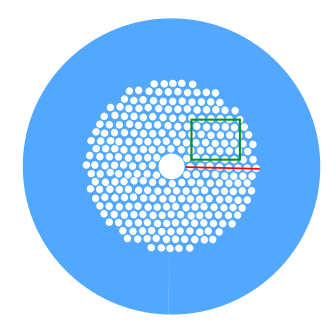
\includegraphics[width=7cm,height=7cm]{./Figures/HCPCF/HCPCF_section.png}}}&
		\subfloat[]{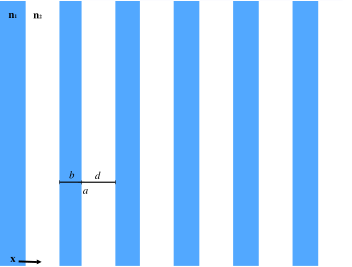
\includegraphics[width=4.5cm,height=3.5cm]{./Figures/HCPCF/HCPCF_1D.png}} \\& 
		\subfloat[]{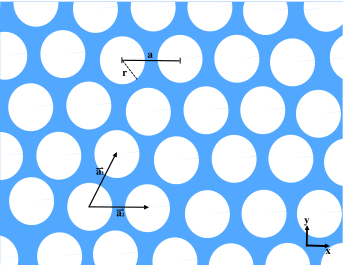
\includegraphics[width=4.5cm,height=3.5cm]{./Figures/HCPCF/HCPCF2D.png}}
	\end{tabular}
	\hfill
	\caption{(a)cross-section of HCPCF highlighting the PC pattern (b)reduced to 1-dimension (2)in 2-dimensions}
	\label{fig:manyD}
\end{figure}

A periodic non-magnetic medium will have repeating dielectric constant\cite{Yariv}
\begin{equation}
	\varepsilon(\boldsymbol{r}) = \varepsilon(\boldsymbol{r}+\boldsymbol{a})  
\end{equation}
Due to its discrete and invariant translational symmetry, the dielectric constant along the medium can be expanded as the Fourier series
\begin{equation}
	\varepsilon(\boldsymbol{r}) = \sum_{\boldsymbol{G}}\varepsilon_{\boldsymbol{G}}e^{i\boldsymbol{G}\cdot\boldsymbol{r}}  
	\label{eqn:fourier_eps}
\end{equation}
where $\boldsymbol{G}$ are the reciprocal lattice vectors such that $\boldsymbol{G}\cdot\boldsymbol{a} = 2\pi n$. We can express the electric field also as the Fourier integral
\begin{equation}
	\boldsymbol{E}(\boldsymbol{r}) = \iiint d^3\boldsymbol{k}\boldsymbol{A}(\boldsymbol{k})e^{i\boldsymbol{k}\cdot\boldsymbol{r}}
	\label{eqn:fourier_E}
\end{equation}
 Using the Maxwell equations (\ref{eqn:maxwell}) the wave equation can be written in terms of the electric field 
 \begin{equation}
 	\begin{aligned}
 	\begin{cases}
 			\vec{\nabla}\times\vec{H} &= -i\omega\epsilon(\vec{r})\vec{E}\\
			\vec{\nabla}\times\vec{E} &= i\omega\mu_0\vec{H}	
 	\end{cases}
 	\end{aligned}
 	\label{eqn:maxwell}
 \end{equation}
\begin{equation}
	\boldsymbol{\nabla}\times(\boldsymbol{\nabla}\times\boldsymbol{E})-\omega^2\varepsilon(\boldsymbol{r})\mu_0\boldsymbol{E} = 0
\end{equation}
Substituting \eqref{eqn:fourier_eps} and \eqref{eqn:fourier_E} into the above results in the dispersion relation:
\begin{equation}
	\boldsymbol{k}\times(\boldsymbol{k}\times\boldsymbol{A}(\boldsymbol{k})) + \omega^2\mu_0\sum_{\boldsymbol{G}}\varepsilon_{\boldsymbol{G}}\boldsymbol{A}(\boldsymbol{k}-\boldsymbol{G}) = 0
	\label{eqn:separation}
\end{equation}
in where for any vector $\boldsymbol{K}$ the solutions of \eqref{eqn:separation} for the coefficient $\boldsymbol{A}(\boldsymbol{K})$ are grouped with the coefficients $\boldsymbol{A}(\boldsymbol{K}-\boldsymbol{G})$, decoupling the coefficients of other vectors that cannot be expressed in the form $\boldsymbol{K}-\boldsymbol{G}$. Disregarding the decoupled vectors, the total electric field can be described as a superposition of normal modes with regard to a chosen vector $\boldsymbol{K}$ :
\begin{equation}
	\boldsymbol{E}_{\boldsymbol{k}}(\boldsymbol{r}) = \sum_{\boldsymbol{G}}\boldsymbol{A}(\boldsymbol{K}-\boldsymbol{G})e^{i(\boldsymbol{k}-\boldsymbol{G})\cdot \boldsymbol{r}}
	\label{eqn:normalmodes}
\end{equation}
we can pull out the Bloch theorem for the electric field from \eqref{eqn:normalmodes}
\begin{equation}
	\boldsymbol{E}_{\boldsymbol{k}}(\boldsymbol{r}+\boldsymbol{a}) = e^{i\boldsymbol{k}\cdot \boldsymbol{a}}\boldsymbol{E}_{\boldsymbol{k}}(\boldsymbol{r})
\end{equation}
\begin{equation}
	\boldsymbol{u_k}(\boldsymbol{r}) = \sum_{\boldsymbol{G}}\varepsilon_{\boldsymbol{G}}e^{i\boldsymbol{G}\cdot\boldsymbol{r}}  
\end{equation}
\begin{equation}
	\varepsilon_{\boldsymbol{G}} = \frac{1}{V}\int d^3\boldsymbol{r}e^{-i\boldsymbol{G}\cdot\boldsymbol{r}}\boldsymbol{u_k}(\boldmath{r})  
	\label{eqn:perm}
\end{equation}
(Expand)  Returning to \eqref{eqn:separation}, can fix $\omega$ to find the corresponding $\boldsymbol{K}$ and normal modes os the system. However, in the case of photonic crystals there are ranges of frequencies that  have no $\boldsymbol{K}$s with real solutions, which implies that waves of these frequencies cannot propagate through the photonic crystal. These non-propagating frequencies are referred to as the photonic band gap.

\subsubsection{1D Photonic Bandgap}
Returning to the 1D periodic stack pictured in \ref{1dstack} the periodicity of dielectric constant is described by $\varepsilon(z) = \varepsilon(z+p)$ where $a = b+d$, the length of one period. The reciprocal lattice vector will be $\boldsymbol{G}_n = n\frac{2\pi}{a}\hat{z}$ and plugging into the Fourier series expansion of $\varepsilon(z)$  from \eqref{eqn:fourier_eps} 
\begin{equation}
	\varepsilon(z)  =\sum_{n=-\infty}^\infty\varepsilon_ne^{in\frac{2\pi}{a}\hat{z}}  
\end{equation}
From the reduction to propagation in the z-direction with the electric field oriented in x-direction, \eqref{eqn:separation} simplifies
\begin{equation}
K^2A(K) + \omega^2\mu_0\sum_{n=-i\infty}^\infty\varepsilon_nA(K-n\frac{2\pi}{a}) = 0
\end{equation}
Expanding the Fourier coefficients to the 1st order and reducing the equations to the dominant coefficients of the form $A(K)$ and $A(K-\frac{2\pi}{a})$ . $|K - g| = K$ and $K = \frac{\pi}{a}$ gives a system of equations that can be solved to find the dispersion relation $\omega(K)$.
\begin{equation}
	\begin{cases}
		\big(K^2-\omega^2\mu_0\varepsilon_{00}\big)A(K) = \omega^2\mu_0\varepsilon_1A(K - g)\\
		\omega^2\mu_0\varepsilon_{-1}A(K) = \big((K-g)^2-\omega^2\mu_0\varepsilon_{00}\big)A(K-g) 
	\end{cases}
\end{equation}
The equations relating these two modes has a solution at
\begin{equation}
		\big(K^2-\omega^2\mu_0\varepsilon_{00}\big)\big((K-g)^2-\omega^2\mu_0\varepsilon_{00}\big) -\big(\omega^2\mu_0\varepsilon_1\big)\big(\omega^2\mu_0\varepsilon_{-1}\big)  = 0 
\end{equation}
 noting $\varepsilon_1 = \varepsilon_{-1}^*$ and $K\approx2g$ simplifies the relationship 
\begin{equation}
	\omega_{\pm}^2 = \frac{K^2}{\mu_0(\varepsilon_{00}\mp|\varepsilon_1|)}
\end{equation}
The dispersion relation has two possible solutions, which specify the top and bottom of the photonic bandgap edges, as illustrated in \ref{fig:1dbp}
\begin{figure}[h]
	\centering
	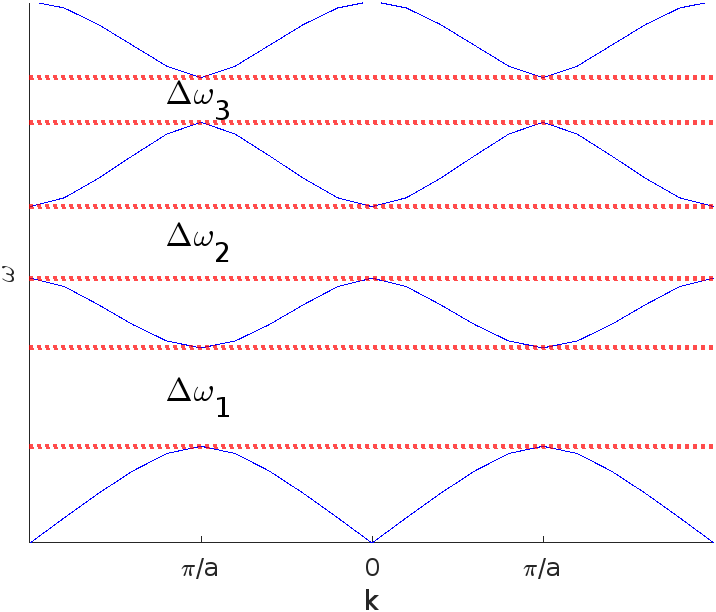
\includegraphics[width=0.6\textwidth]{./Figures/HCPCF/1D_BandGap.png}
	\caption {Band plot for a 1D photonic crystal with parameters-,-, solved using Finite Difference Time Domain(FDTD) method\cite{sukhoivanov}.}
	\label{fig:1dbp}
\end{figure}

If solving for the wavevector at a frequency between $\omega_{\pm}$, only complex solutions will exist. This means that only evanescent waves, not electromagnetic waves, propagate through the medium while the electromagnetic waves are reflected back; the medium acts as a mirror for the bandgap wavelengths.\\
This is the the phenomenon that allows for HCPCF to guide certain frequencies of light: wavelengths in the bandgap are reflected by surrounding Bragg Grating confining them to the core of the fiber, while the rest are allowed to propagate through the grating. 

\subsubsection{2D Photonic Bandgap}
To understand the full picture of  light propagation in hollow-core fiber, we need to expand to the 2D case pictured in  \ref{fig:manyD}c. However, with the electromagnetic waves now propagating in two dimension there is an added layer of complexity with the TE TM wave polarizations and the bandgaps. In addition to controlling the refractive index of the material and the period of the lattice, the lattice structure and hole radius will affect the performance of the photonic crystal, the latter playing a large role in the completeness of the photonic bandgap.  In the 2D photonic crystal, the in-plane guided modes will have either magnetic fields in-plane and electric fields perpendicular to the lattice (TE modes)  or electric fields in-plane and magnetic fields perpendicular to the lattice ( TM modes) . As the TE and TM modes are perpendicular to each other they may exhibit wildly different dispersion relations, which means that an optical bandgap is not guaranteed to persist for all polarizations\cite{joannopoulos}. This is certainly the case for square lattice phonic crystals, but  other patterns such as the honeycomb (which is the structure in our HCPCF)  do have a bandgap persisting for all all polarizations\cite{villeneuve}. This all to say, it is important to consider all polarization effects when making decisions about photonic crystal patterns for two or more dimensions. \\
\begin{figure}[h]
	\centering
	\foreach \x in {HCPCF_2D_cartesian, HCPCF_2D_reciprocal}
	{ 
		\begin{subfigure}[b]{0.45\textwidth}
			\includegraphics[width=\textwidth]{./Figures/HCPCF/\x.png}
			\caption{}
		\end{subfigure}
		\hfil
	}
	\caption {(a) primitive lattice vectors and (b) primitive reciprocal lattice vectors with first Brillouin zone (green) and irreducible  Brillouin  zone (red) depicted for a honeycomb lattice structure.  }
	\label{fig:2d}
\end{figure}
\clearpage
Considering the lattice structure in \ref{fig:2d}(a), and taking propagation in the xy-plane ($K_z=0$ and $z=0$ for simplicity), the wavevector and position vectors reduce to  $\boldsymbol{K_{||}}=k_x\hat{x}+k_y\hat{y}$ and $\boldsymbol{r_{||}}=x\hat{x}+y\hat{y}$.  The primitive lattice vectors of a honeycomb photonic crystal will be:
\begin{equation}
	\boldsymbol{a}_1 = a\hat{x} \hspace{1cm} \boldsymbol{a}_2 = \frac{a}{2}\hat{x}+\frac{a\sqrt{3}}{2}\hat{y}
\end{equation}
and transforming to the momentum-space,  $\boldsymbol{b}\cdot\boldsymbol{a} = 2\pi\delta_{ij}$, as shown in \ref{fig:2d}(b) the primitive reciprocal lattice vectors are
\begin{equation}
	\boldsymbol{b}_1 = \frac{2\pi}{a}\hat{x}-\frac{2\pi}{a\sqrt{3}}\hat{y} \hspace{1cm} \boldsymbol{b}_2 =\frac{4\pi}{a\sqrt{3}}\hat{y} 
\end{equation}
Taking these in combination of $n, m$ integer scaling factors, the reciprocal lattice vector is defined $\boldsymbol{G_{||}} = n\boldsymbol{b}_1 + m\boldsymbol{b}_2$. 
The electromagnetic field defined for a two dimensional system
\begin{equation}
	\boldsymbol{E}(\boldsymbol{r}) = e^{i\boldsymbol{k}\cdot\boldsymbol{r}}
	\sum_{m=-\infty}^\infty\sum_{n=-\infty}^\infty\boldsymbol{E}_{m,n}
	e^{i(n\boldsymbol{b_1}+m\boldsymbol{b_2})\cdot\boldsymbol{r}}
		\label{eqn:2d_emf}
\end{equation}
and the correlating Fourier expansion of dielectric function \eqref{eqn:perm}
\begin{equation}
	\varepsilon_{\boldsymbol{G_{||}}} = \frac{1}{a'\cdot b'}\int dxdye^{i(G_xx + G_yy)}\boldsymbol{u_k}(x, y)  
	\label{eqn:2d_perm}
\end{equation}
are substituted into \eqref{eqn:maxwell}. 
Utilizing the lattice symmetry and periodicity, the problem can be restricted to only solve for Bloch modes inside the of the irreducible Brillouin zone.
The first Brillouin zone is defined by the perpendicular bisectors to the primitive reciprocal lattice vectors, depicted in green in \ref{fig:2d}(b) and can be further subdivided into the irreducible Brillouin zone shown in red. 
In order to find the photonic bandgap, solving the dispersion equation just along the irreducible Brillouin zone is sufficient.
For a honeycomb lattice, the $k$-path to follow would be
\begin{equation}	
	\begin{cases}
		|\Gamma X| = \frac{2\pi}{a\sqrt{3}}, &k_x=0, 0<k_y<\frac{2\pi}{\sqrt{3}a}\\
		|XJ| =  \frac{2\pi}{3a}, &0<k_x<\frac{2\pi}{3a}, k_y=\frac{2\pi}{\sqrt{3}a}\\
		|\Gamma J| = \frac{4\pi}{3a}, & 0<k_x<\frac{2\pi}{3a}, k_y=\sqrt{3}k_x
	\end{cases}
\end{equation}
Discretizing  (\ref{eqn:2d_emf}) and (\ref{eqn:2d_perm}) then picking a few points along the $k$-path, numerical methods can be used to solve for the optical bandgap. \ref{fig:2dbp} shows the resulting TE bandgap for a honeycomb lattice with parameters-,-, using Plane Wave Expansion(PWE)\cite{sukhoivanov}. 
\begin{figure}[h]
	\centering
			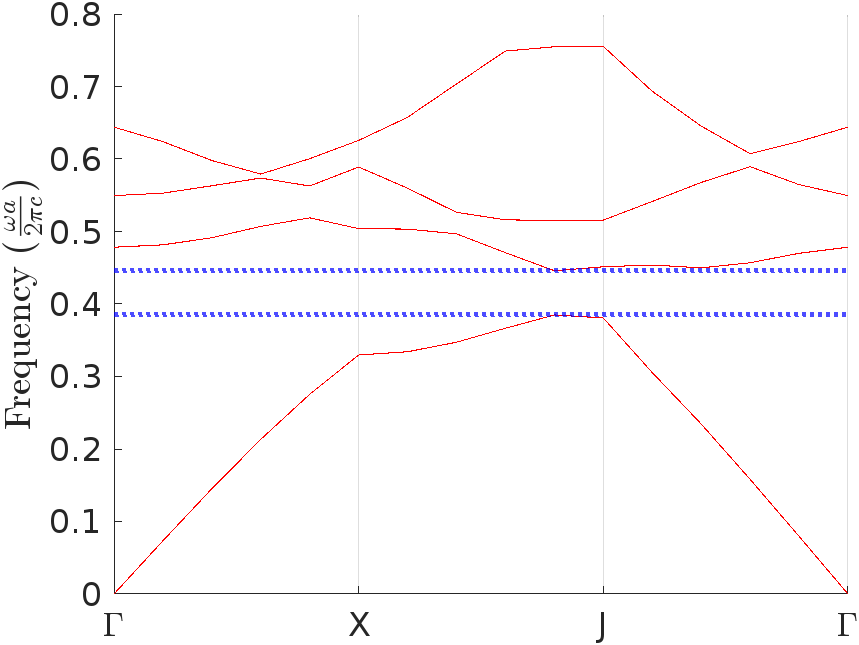
\includegraphics[width=0.8\textwidth]{./Figures/HCPCF/2D_BandDiagram.png}
	\caption {Band plot along the irreducible Brillouin zone for a honeycomb lattice with parameters -,-, . Solved for using Plane Wave Expansion(PWE) numerical method\cite{sukhoivanov}.} 
	\label{fig:2dbp}
\end{figure}

\clearpage
\subsection{Bandgap Shift}
The modal magnetic field distributions satisfy:
\begin{equation}
	(\nabla^2_t + k^2n(\boldsymbol{r})^2 - \beta)\boldsymbol{H(r)} = (\nabla_t\times\boldsymbol{H(r)})\times(\nabla_t ln(n(\boldsymbol{r})^2))
\end{equation}
This equation gives a scaling law for absolute refractive index at fixed contrast: 
``a solution for a transverse scale represented by $\Lambda$is replicated in an identical structure with a different $\Lambda$ if the wavelength is scaled proportionately, to keep $k\Lambda$ constant''\\
``We emphasise that the scalar wave equation (and therefore the scaling laws derived from it) is accurate for the smallest index contrasts only. However, for step-index structures the vector term in Eq. (2) only exists at boundaries, so the scalar wave equation accurately represents wave propagation elsewhere. Since bandgaps arise from interference and resonance effects among such generic waves, the scaling laws of Eq. (5) should be at least approximately valid'' ~1.45 RI contrast\cite{birks}

Scaling law for the wave equation for the transverse coordinates
$X=x\Lambda^{-1}$ $Y=y\Lambda^{-1}$
where $\Lambda$ is a solution to the transverse scale. 
\begin{equation}
	n(X, Y) = \begin{cases}
		1, &n_1 \text{   (high RI)}\\
		0, & n_2 \text{   (low RI)}
	\end{cases}
\end{equation}
normalized scaled wave equation:
\begin{equation}
	\nabla_\perp^2\Psi + (v^2n(X, Y) - w^2)\Psi = 0
\end{equation}
With $\nabla_\perp = \partial^2/\partial X^2 + \partial^2/\partial Y^2 $
solving for the frequency parameter $v^2$ and eigenvalue $w^2$:
\begin{equation}
	\begin{aligned}
		v^2  &= \Lambda^2k^2(n_1^2 - n_2^2)\\
		w^2 &= \Lambda^2(\beta^2 - k^2n_2^2)
	\end{aligned}
\end{equation}
from the equation above we see that the $w^2$ is determined by the frequency parameter $v^2$ and the index distribution function $n(X, Y)$.
This implies that $w^2$ and $v^2$ are invariant with changes to the parameters $k, \Lambda, n_1, n_2$. 
$k = \omega/c$ $\beta = kcos\theta$ longitudinal component of the wavevector. Because the light propagates along the fiber, much of its wavevector is taken up by the longitudinal component. 

In the HCPCF case where the glass refractive index is held constant and the air in the fiber is replaced by a new material the equations can be rewritten with $n_1 = n_{glass}$ and $n_2 = n_{air}=1$:
\begin{equation}
	\begin{aligned}
		v^2 - w^2 &= \Lambda^2(k^2n_{glass} - \beta^2)\\
		v &= k\Lambda n_{glass}\sqrt{n_{air} - \frac{n_{air}}{n_{new}}}
	\end{aligned}
\end{equation}
The initial index contrast $N_0 = \frac{n_{air}}{n_{glass}}$ moves to$ N = \frac{n_{new}}{n_{glass}}$ with the change in RI $n_{air} <  n_{new} < n_{glass}$
This leads to the new center bandgap to be governed by the equation: 
\begin{equation}
	\lambda = \lambda_0\sqrt{\frac{1-N^{-2}}{1-N_0^{-2}}}
\end{equation}
This has been experimentally confirmed to hold for HCPCF \cite{antonopoulos}.





%======================================================================
\chapter{Liquid-Filled HCPCF}
%======================================================================
In this chapter follows a background on different filling methods, the integrity of the scaling laws, and transmission of liquid-filled HCPCF.
\section{Experimental Set-Up}
\begin{figure}[!htb]
	\centering
	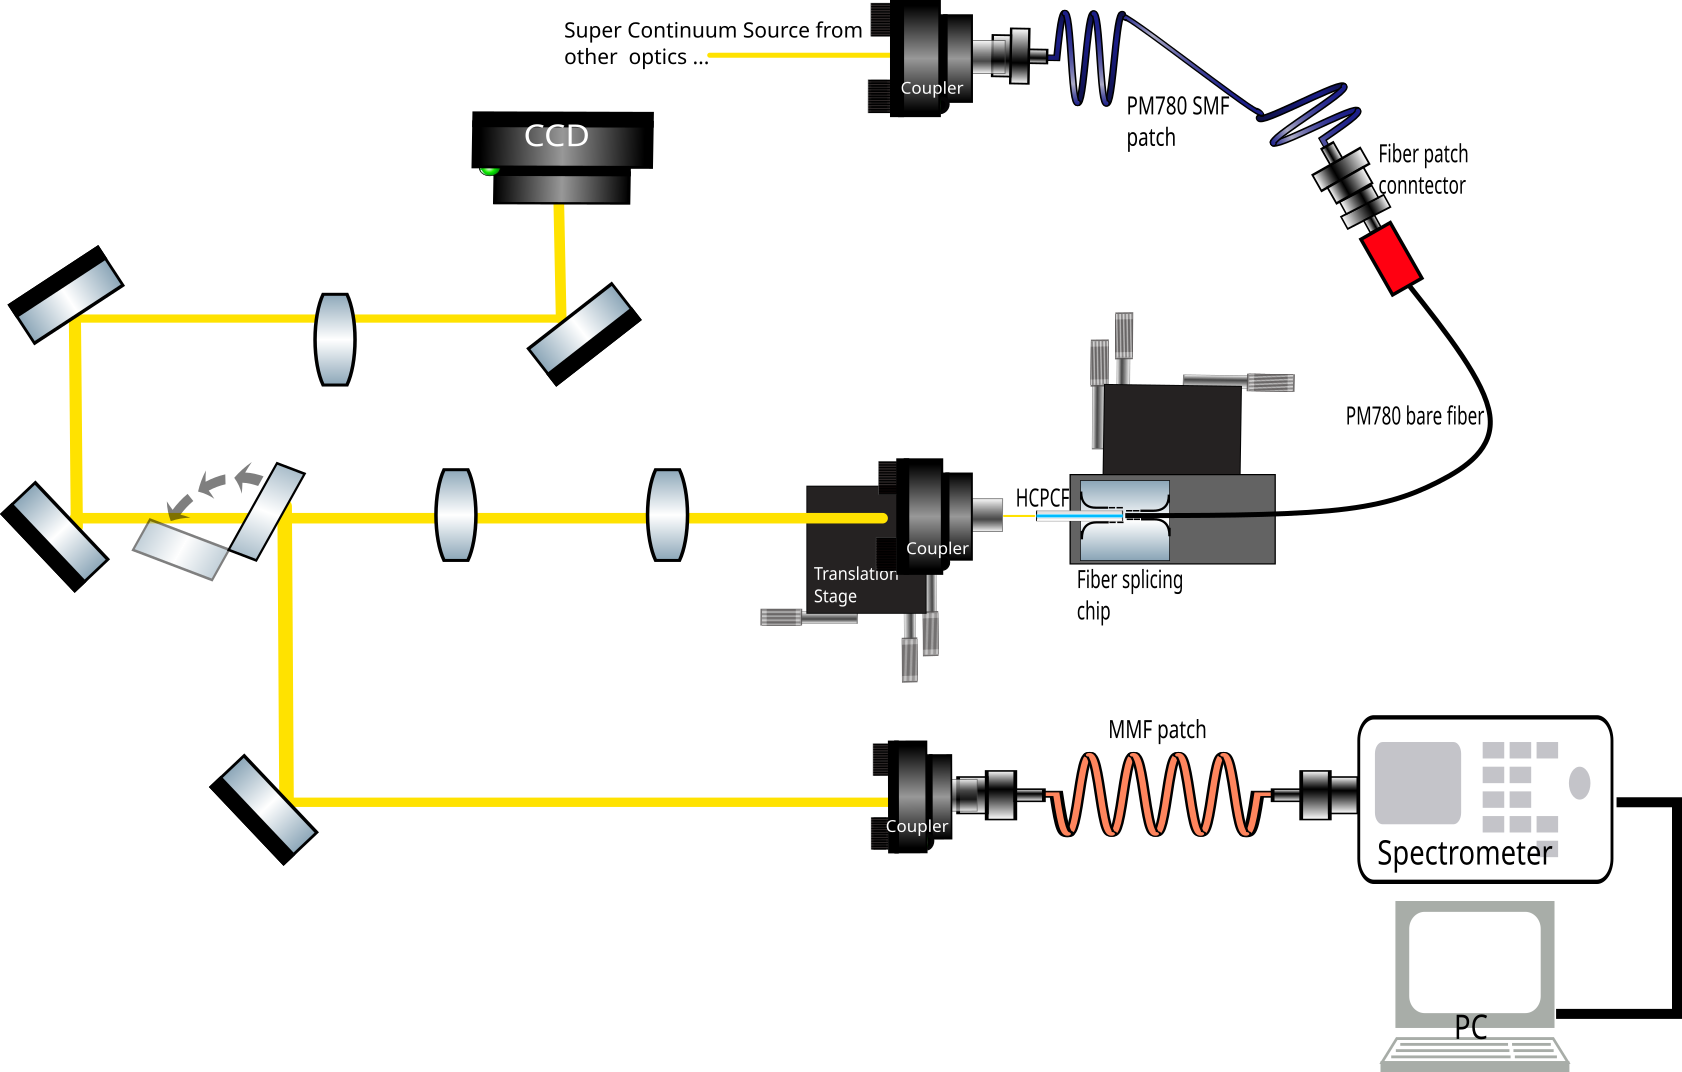
\includegraphics[width=0.6\textwidth]{./Figures/fiberfilling/Transmission_SetUp.png}
	\caption{Fiber transmission experimental set-up. The path to the CCD camera is used to monitor the modeshape coming out of the fiber and the path to the spectrometer is used to measure the transmission spectrum of the fiber.}
	\label{fig:filling exp}
\end{figure}
For the transmission measurements, shown in Fig.\ref{fig:filling exp}, fibers were cut to be between 6cm and 8cm in length. To ensure consistent coupling and positioning, light was coupled to the core of the fiber by connecting to a solid-core PM780HP fiber via a mechanical splicing chip \cite{maruf}.\\
In our experiments two different filling methods are tested: full fiber filling, and selective filling, as well as two filling liquids: deionized water (which will be referred to as DI Water or H${}_2$O) and heavy water D${}_2$O.
\begin{figure}[!htb]
	\centering
	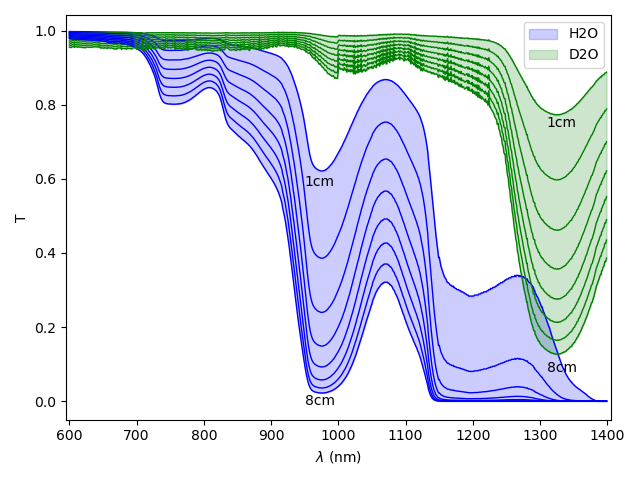
\includegraphics[width=0.6\textwidth]{./Figures/fiberfilling/water_transmission/water_transmission.png}
	\caption{The transmission of heavy water(green) and regular water(blue) is shown for slabs of thickness ranging from 1cm to 8cm in increments of 1cm using absorption data by \cite{kedenburg}. }
	\label{fig:water transmission}
\end{figure}
Fibers that are fully-filled with water will produce a frequency shift in the bandgap. On the other hand, when the core is selectively filled with water, the core refractive index will be greater than effective refractive index of the cladding and light will be guided via total-internal reflection. H${}_2$O, while widely available and a common solvent, has high absorption loss in the near infrared (NIR) but its most common isotope D${}_2$O has comparatively much less absorption loss in the same region (Fig.\ref{fig:water transmission}). The transmission in HCPCF are explored for H${}_2$O for its ubiquity while D${}_2$O for its suitability as a filling liquid in the NIR.
\subsection{Selective Filling}
\subsubsection{Filling Method}
To selectively fill the core of 800nm HCPCF, the photonic crystal cladding was collapsed while leaving the hollow-core open and is similarly filled with liquid using capillary action. The cladding is collapsed by placing the HCPCF opposite of a solid-core fiber in a fusion splicer \cite{xiao} and adjusting arc current duration and power to melt the cladding structure while remaining distanced enough to prevent fusion with the solid-core fiber.
\begin{figure}[!htb]
	\centering
	\foreach \x in {50ms 15mA, 70ms 20mA, 70ms 25mA, 80ms 25mA, 90ms 25mA, 100ms 25mA}
	{
		\begin{subfigure}[b]{0.3\textwidth}
			\includegraphics[width=\textwidth]{./Figures/fiberfilling/arc_power/\x.png}
			\caption{\x}
		\end{subfigure}
		\hfil
	}
	\caption{Side profile of collapsed cladding 1550HC fiber running the fiber splicer with varying current strength and duration. }
	\label{fig:selective filling}
\end{figure}
In Fig.\ref{fig:selective filling} the extent of collapse of the cladding is compared to various timing and power for an ORIENTEK T40 fusion splicer. The optimal setting is around an arc power of 25mA for a 70ms duration, though due to the imprecision in the arc power discharge the cladding on occasion will be overexposed, as shown in Fig.\ref{fig:selective err}.

\begin{figure}[!htb]
	\centering
	\foreach \x in {collapsed, fiberend}
	{
		\begin{subfigure}[b]{0.4\textwidth}
			\includegraphics[width=\textwidth]{./Figures/fiberfilling/arc_err/\x.jpg}
		\end{subfigure}
		\hfil
	}
	\caption{Variation between fibers using splicer settings 70ms 25ms  }
	\label{fig:selective err}
\end{figure}
\subsubsection{Transmission}
\begin{figure}[!htb]
	\centering
	\foreach \x in {HC800\_empty, HC800\_D2O, HC800\_H2O}
	{
		\begin{subfigure}[b]{0.32\textwidth}
			\includegraphics[width=\textwidth]{./Figures/fiberfilling/HC800/ModeShape/\x.png}
			\caption{}
		\end{subfigure}
		\hfil
	}
	\caption{Modeshape of 800 hollow-core fiber filled with (a)air (b)heavy water (c)DI water.}
	\label{fig:800 modeshape}
\end{figure}
\begin{figure}[!htb]
	\centering
	\includegraphics[width=0.75\textwidth]{./Figures/fiberfilling/HC800/transmission.png}
	\caption{Transmission of H${}_2$O and D${}_2$O in a selectively-filled 800nm hollow-core fiber.}
	\label{fig:trans 800hc}
\end{figure}
The air-filled 800nm HCPCF covers a transmission spectral range of 750nm–950nm. Light exits the fiber with a Gaussian mode shape, as shown in Fig.\ref{fig:800 modeshape}. In a H${}_2$O core, the coupling efficiency of the fiber drops to 31\%, while a heavy water filled core is less affected by absorption over this region and retains a coupling efficiency of up to 67\%.
\subsection{Full-Fiber Filling}
\subsubsection{Filling Method}
The air in 1550nm HCPCF was replaced with deionized water and heavy water by utilizing capillary action. 
\subsubsection{Transmission}
\begin{figure}[!htb]
	\centering
	\foreach \x in {HC1550_empty, HC1550_full_D2O, HC1550_H2O}
		{
			\begin{subfigure}[b]{0.32\textwidth}
				\includegraphics[width=\textwidth]{./Figures/fiberfilling/HC1550/ModeShape/\x.png}
				\caption{}
			\end{subfigure}
			\hfil
		}
	\caption{Modeshape of 1550 hollow-core fiber filled with (a)air (b)heavy water (c)DI water. Fiber filled with heavy water maintains a Gaussian profile while the fiber with regular distilled water shows some distortion.}
	\label{fig:1550 modeshape}
\end{figure}
The air-filled 1550nm HCPCF covers a transmission spectral range of 1200nm–1700nm. With a filled core and cladding, the spectral range shifts to transmitting wavelengths between 600nm–1100nm for both heavy water and water, confirming the scaling laws. Heavy water achieved a coupling efficiency of 47\%, but water only 16\%. While the D${}_2$O fiber modeshape retains a Gaussian profile, the H${}_2$O mode shape contains noise as some light also leaks from the photonic structure. The absorption effects of H${}_2$O severely reduce the transmission for wavelengths above 820nm, while compares well to the transmission of the D${}_2$O fiber below 820nm and could arguably be used as a filling liquid.
\begin{figure}[!htb]
	\centering
	\includegraphics[width=0.75\textwidth]{./Figures/fiberfilling/HC1550/transmission.png}
	\caption{Transmission of H${}_2$O and D${}_2$O in fully-filed and core-filled 1550nm hollow-core fiber.}
	\label{fig: trans 1550hc}
\end{figure}
\clearpage


\section{Indocyanine Green}
Due to the difficultly in isolating single-chirality solutions of CNTs, as outlined in in the previous chapter, indocyanine green (ICG) - a fluorescent dye often used in microscopy imaging\cite{farrakhova, spartalis} - was initially used in place of CNTs in the fiber.  This particular dye is an organic semiconductor with Homo-Lumo gap calculations estimating a $~2$eV energy gap, with variations depending on the solvent\cite{Fang}. The HOMO and LUMO energy levels in organic semiconductors are parallel to the maximum valence and minimum conduction, and the aforementioned energy gap falls within the range of energy bandgaps found in inorganic semiconductors. 
\begin{figure}[h]
	\centering
	\foreach \x in {Homo_Lumo, chemical_formula}
	{ 
		\begin{subfigure}[b]{0.45\textwidth}
			\includegraphics[width=\textwidth]{./Figures/ICG/\x.png}
			\caption{}
		\end{subfigure}
		\hfil
	}
	\caption{(a) Depiction of the Homo-Lumo gap in organic semiconductors and the transition occurring between ground and excited states. (b) The chemical structure of ICG provided by MP Biomedicals. }
	\label{fig:homolumo}
\end{figure}
\clearpage
The following section details the the optical properties of ICG and measurements of the optical properties when confined in HCPCF. 

\subsubsection{ Absorption Cross-Section}
The absorption is largely bimodal, with peak excitation at 780nm and 700nm, but transforms into a monomeric distribution at 780nm at low concentrations and 700nm at high concentrations. 
\begin{figure}[h]
	\centering
	\foreach \x in {D2O_acs, H2O_acs}
	{ 
		\begin{subfigure}[b]{0.49\textwidth}
			\includegraphics[width=\textwidth]{./Figures/ICG/\x.png}
			\caption{}
		\end{subfigure}
		\hfil
	}
	\caption{ Absorption cross-section at peak wavelengths 700nm(blue) and 780nm(green) for ICG dissolved in D2O(a) and H2O(b) .  Data from (cite) was fitted using a linear regression model. }
	\label{fig:icg abs plots}
\end{figure}
Due to the chemical formation of ICG, the absorption of the molecule when dissolved in a solvent is highly concentration-dependent. ICG is made up of monomers, which are a type of molecule that can react with other monomers to form polymer chains. In the case of ICG, its monomers react with each other to form dimers, a chain of two join monomers. With higher concentrations, monomers are closer in proximity and the molecules are more likely shift from monomers to dimers which are less likely to be excited and shift the center absorption wavelength. The concentration of monomer $M$ to dimmers $D$ is governed by the equilibrium reaction
\begin{equation}
	M+M\rightleftarrows D
\end{equation}
and law of mass action relation concentration 
\begin{equation}
	[D] =  K_D[M]^2
\end{equation}
Where $K_D$ is the dimmerization constant . Written in terms of concentration $C$ and mole fractions, $[M] = x_MC= (1-x_D)C $ and $[D]=\frac{x_D}{2}C$., the  mole fraction of dimmers can be written in terms of the dimmerization constant and concentration.
\begin{equation}
	x_D = 1 + \frac{1}{4K_DC} - \sqrt{\big( 1 + \frac{1}{4K_DC}\big)^2-1}
	\label{xd}
\end{equation}
 The absorption cross-section model for ICG\cite{mauerer, philip} will be an average of the affects of the of monomers and dimmers, where d $\sigma_M$ and $\sigma_D$ are the monomer and dimer absorption cross-sections respectively.
\begin{equation}
	\sigma = x_M \sigma_M + x_D \sigma_D = \sigma_M - x_D(\sigma_M - \sigma_D)
	\label{abc}
\end{equation}
Plugging (\ref{xd}) into (\ref{abc}), remaining parameters could be found by doing a linear regression fit to absorption cross-section vs. concentration data from literature and the expected absorption cross-section could be calculated for any concentration. For ICG dissolved in H2O, the existing literature has some variation and so the upper/lower bounds and average were taken, while little data was available for ICG dissolved in D2O. The behavior in H2O and D2O are quite similar and are plotted in Fig\ref{fig:icg abs plots}. At lower concentrations the absorption cross-section is slightly greater for D2O than H2O, with the reverse for high concentrations. 
\clearpage
\begin{table}
	\centering
	\begin{tabularx}{0.8\textwidth} { 
		| >{\centering\arraybackslash}X 
		| >{\centering\arraybackslash}X 
		| >{\centering\arraybackslash}X 
		| >{\centering\arraybackslash}X | }
		\hline
		$\lambda_{peak} = 780nm$ & $K_D$ & $\sigma_M$ & $\sigma_D$\\
		\hline
		\cite{holzer} & $6.01x10^5$ & $9.29x10^{-16}$ & $2.28x10^{-16}$\\
		\hline
		\cite{landsman} & $1.03x10^5$ & $6.74x10^{-16}$ & $1.54x10^{-16}$\\
		\hline
		\cite{mauerer} & $1.40x10^5$ & $6.72x10^{-16}$ & $1.11x10^{-16}$\\
		\hline
		Average & $3.06x10^6$ & $7.94x10^{-16}$ & $1.72x10^{-16}$\\
		\hline
	\end{tabularx}
	\captionof{table}{Absorption Cross Section parameter fitting of ICG  dissolved in deionized water. Fitting done with linear regression on $\sigma$ vs. concentration data measured at $\lambda=780nm$ from  literature. \label{h2o780}}
\end{table}
\begin{table}
	\centering
	\begin{tabularx}{0.8\textwidth} { 
		| >{\centering\arraybackslash}X 
		| >{\centering\arraybackslash}X 
		| >{\centering\arraybackslash}X 
		| >{\centering\arraybackslash}X | }
		\hline
		$\lambda_{peak} = 700nm$ & $K_D$ & $\sigma_M$ & $\sigma_D$\\
		\hline
		\cite{holzer} & $3.00x10^3$ & $2.29x10^{-16}$ & $25.68x10^{-16}$\\
		\hline
		\cite{mauerer} & $3.06x10^4$ & $8.89x10^{-16}$ & $3.93x10^{-16}$\\
		\hline
		Average & $9.31x10^3$ & $1.62x10^{-16}$ & $4.74x10^{-16}$\\
		\hline
	\end{tabularx}
	\captionof{table}{Absorption Cross Section parameter fitting of ICG  dissolved in deionized water. Fitting done with linear regression on $\sigma$ vs. concentration data at $\lambda=700nm$ from literature. \label{h2o700}}
\end{table}	
\begin{table}
	\centering
	\begin{tabularx}{0.8\textwidth} { 
		| >{\centering\arraybackslash}X 
		| >{\centering\arraybackslash}X 
		| >{\centering\arraybackslash}X 
		| >{\centering\arraybackslash}X | }
		\hline
		$\lambda_{peak}$ & $K_D$ & $\sigma_M$ & $\sigma_D$\\
		\hline
		$780nm$ & $3.22x10^4$ & $7.14x10^{-16}$ & $2.68x10^{-17}$\\
		\hline
		$700nm$ & $1.67x10^4$ & $2.833x10^{-16}$ & $6.28x10^{-16}$\\
		\hline
	\end{tabularx}
	\captionof{table}{Absorption Cross Section parameter fitting of ICG  dissolved in heavy water. Fitting done with linear regression on $\sigma$ vs. concentration data at $\lambda=700nm$ from literature. \label{d20700780}}
\end{table}
\clearpage

\subsubsection{ Photostability}
At high concentrations, ICG behaves as a  "J-aggregate", a category of dyes that have a shift in absorption band to larger wavelengths in certain solvents. When mixed into water and other solvents, ICG shifts over time to a center wavelength of 893nm. This process can be accelerated under high heat in high-concentration (in the range of 1000ppm solutions) forms \cite{rotermund},  J-aggregates can be stored at room temperature for several months. However, at such a state the dye will be too optically dense to observe any optical excitation and when diluted to perform such measurements, the J-aggregates will begin to detach into smaller molecules within 24hrs.  The effects of dye concentration of storage life in aqueous solutions becomes a tricky balance at single-digit ppm concentrations, where the fluorescence intensity of the dye is at its greatest but with degradation to undetectable levels occurring in a couple of hours at best if in optimal storage conditions\cite{landsman, saxena}. The rate of deterioration occurs so linearly based on the initial concentration of ICG\cite{holzer}, but the amount of light exposure of the solution will also exasperate the degradation rate\cite{saxena}. 
\begin{figure}[h]
	\centering
	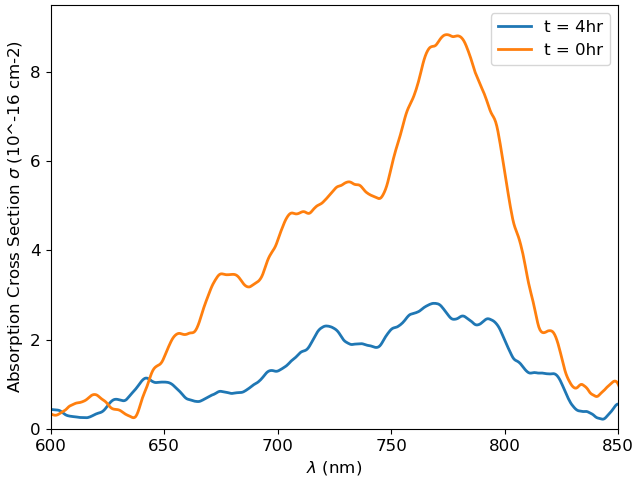
\includegraphics[width=0.6\textwidth]{./Figures/ICG/abc_time.png}
	\caption{Degradation of a 4.5ppm initial concentration sample after 4hrs of light exposure reduced to a 2ppm concentration.}
	\label{fig:icgphoto}
\end{figure}
\clearpage


\subsubsection{ Fluorescence}
The peak emission wavelength for ICG varies within 800nm-820nm\cite{philip, saxena} when excited at 780nm and decreases as solution concentration increases, The dimmerization effects are attributed to (a) The formation of weakly fluorescent ICG molecular aggregates at high concentrations (b) self-quenching and (c) re-absorption of the emitted fluorescence by the ICG molecules due to overlap of the absorption and emission spectra. In the J-aggregate form  the excitation wavelength shifts to 834nm and the emission peak at 890nm, however, low quantum yield and strong light scattering does not lend to accurate measurements\cite{rotermund}.  
\begin{figure}[!htb]
	\centering
	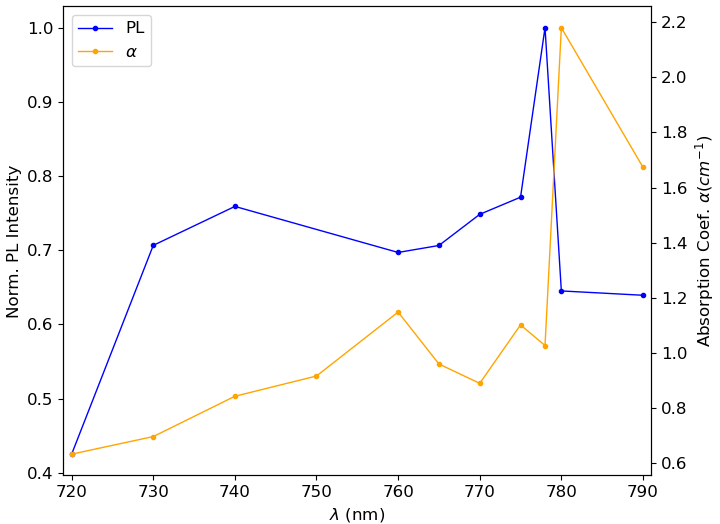
\includegraphics[width=0.6\textwidth]{./Figures/ICG/wl_fluor_absp.png}
	\caption{ Maximum fluorescence and maximum absorption spectrum of 4.5ppm initial concentration sample.}
	\label{fig:i}
\end{figure}
At the maximum absorption wavelength the power is increased to find the maximum faction of fluorescence and saturation point of the absorption. 
\begin{figure}[!htb]
	\centering
	\foreach \x in {power_fl_absp, fl_absp}
	{ 
		\begin{subfigure}[b]{0.47\textwidth}
			\includegraphics[width=\textwidth]{./Figures/ICG/\x.png}
			\caption{}
		\end{subfigure}
	}
	\caption{(a) QY=0.05\% (b) }
	\label{fig:icg_power}
\end{figure}
\clearpage
\subsection{Fiber Absorption Effects}
For calculations of optical density within the HCPCF, the core radius will be  $r_{core} = 5\pm 0.05\mu m$ with beam waist $w_0 = 4.5 \pm 0.05\mu m$ for 1550nm HCPCF and $r_{core} = 3.75 \pm0.05\mu m$ with beam waist $w_0 = 2.75 \pm 0.05$. For ICG dispersed in water, molecule aggregate radii have been measured between $2nm - 200nm$ \cite{dedora} with J-aggregates forming at radii $>50nm$\cite{weigand}. Due to the low concentration samples of dye used in out experiments, the lower range of molecule diameter is used, meeting the Raleigh scattering approximation condition $\frac{2\pi r}{\lambda} <<1$, the scattering cross-section is 
\begin{equation}
	\sigma_0 = \frac{2\pi^5 (2r_{particle})^6}{3\lambda^4}(\frac{N^2 -1}{N^2+2})^2
	\label{raleigh}
\end{equation}
where $N=\frac{n_{particle}}{n_{solvent}}$. Applying the parameters above and  (\ref{raleigh}) to (\ref{OD}) the estimated concentration of ICG molecules for optically dense medium ($OD_{fiber}=1$) has a range of $N_{particle} = 1.5\times 10^8 \sim 2.0\times 10^{14}$ molecules and $N_{particle} = 8.2\times 10^7 \sim 1.1\times 10^{14}$ molecules for 1550nm and 800nm HCPCF respectively varying the ICG aggregate radii within the approximation condition. \\

Low-concentration samples of dye were prepared and filled a 800nm HCPCF core and 1550nm HCPCF core and cladding. The absorption spectrum of the dye was detected, though muddled by additional losses from the fiber, as shown in Fig. \ref{fig:icg_absp}. Additionally, there is an observed 18nm shift in the peak absorption from 778nm to 796nm in the 1550nm bandgap-shifted liquid-filled fiber, while the 800mn liquid-core fiber has an insignificant 4nm shift in peak from 775nm to 771nm.  
\begin{figure}[!htb]
	\centering
	\foreach \x in {absp_800hc, absp_1550hc}
	{ 
		\begin{subfigure}[b]{0.49\textwidth}
			\includegraphics[width=\textwidth]{./Figures/ICG/\x.png}
			\caption{}
		\end{subfigure}
		\hfil
	}
	\caption{ Absorption spectrum of ICG samples (a) 2.5 ppm concentration in core of 800nm HCPCF and (b)  4 ppm concentration in core and cladding of 1550nm HCPCF. }
	\label{fig:icg_absp}
\end{figure}
\clearpage
Fluorescence was guided in the bandgap-shifted 1550nm HCPCF, but not in the 800nm core-filled HCPCF. It is suspected that the narrow bandgap of the 800nm HCPCF in combination with lower refractive index contrast cam into play; the absorption loss in the waveguide reduced excitation and the re-absorption effects of the overlapping excitation-emission spectra were greater than the number of emitted photons. \\
For the 4ppm ICG sample the ratio of emitted photons to the input number of photons at the excitation wavelength are compared in Fig. \ref{fig:icg_fluor}, with the fraction of fluorescence in 1550nm HCPCF $\sim35$x greater than that measured through the cuvette.
\begin{figure}[!htb]
	\centering
	\foreach \x in {diff_max_pl, OD, fluor_1550hc, fluor_cuvette}
	{ 
		\begin{subfigure}[b]{0.47\textwidth}
			\includegraphics[width=7cm,height=5.5cm]{./Figures/ICG/\x.png}
			\caption{}
		\end{subfigure}
	}
	\caption{(a) The maximum fractional fluorescence is plotted against excitation wavelength for a 4ppm ICG sample in a 1cm piece of 1550nm HCPCF and 1cm cuvette. The maximum fractional fluorescence of the ICG in the cuvette is only 4\% of that measured in fiber. (b)  The optical density at each excitation wavelength. The fractional fluorescence spectrum of the 4ppm ICG solution in (c) 1550nm HCPCF (d) a cuvette. }
	\label{fig:icg_fluor}
\end{figure}

For the $L_{fiber}=1cm$  piece of fiber, the number of molecules contained in a perfectly filled core will be
\begin{equation}
	N_{particle} = M_{ICG}*C*V_{fiber}=\frac{1 mol}{774.98g}*\frac{4mg}{1L}*\pi(5\mu m)^2(1cm) = 2.441\times10^9 molecules
\end{equation} 
Using the measured optical density in the fiber, Fig. \ref{fig:icg_fluor}b the estimated radius of the aggregate ICG molecules is $r_{particle} = 13.7 \pm 0.2nm$.  

\clearpage

\subsection{Experiment Set-Up}

Preparation
1. Stock
1) Using the micropipette, measure 1ml of D2O or H2O into a vial 
2) Using the scale, measure 1mg of ICG powder
3) Pour the measured ICG into the 1ml of D2O/H2O
4) Close the vial and shake for 15 seconds to dissolve

2. Dilution
1) Measure 5ml of D2O or H2O into a vial 
2) Using the pipette, measure 10ul of the stock solution
3) Output the 10ul of stock solutions into the 100ml of D2O/H2O
4) Close the vial and shake for 15 seconds to dissolve
Used within 12 hrs of creation

\subsection{ICG in HCPCF}
Low-concentration samples of dye were prepared and filled a 800nm HCPCF core and 1550nm HCPCF core and cladding. The absorption spectrum of the dye was detected, though muddled by additional losses from the fiber, as shown in Fig. \ref{fig:icg_absp}. Additionally, there is an observed 18nm shift in the peak absorption from 778nm to 796nm in the 1550nm bandgap-shifted liquid-filled fiber, while the 800mn liquid-core fiber has an insignificant 4nm shift in peak from 775nm to 771nm.\\ 
\begin{figure}[!htb]
	\centering
	\foreach \x in {absp_800hc, absp_1550hc}
	{ 
		\begin{subfigure}[b]{0.49\textwidth}
			\includegraphics[width=\textwidth]{./Figures/ICG/\x.png}
			\caption{}
		\end{subfigure}
		\hfil
	}
	\caption{ Absorption spectrum of ICG samples (a) 2.5 ppm concentration in core of 800nm HCPCF and (b)  4 ppm concentration in core an
		d cladding of 1550nm HCPCF. }
	\label{fig:icg_absp}
\end{figure}
For 800nm core-filled HCPCF, ICG solutions were prepared with H${}_2$O and  D${}_2$O solvents, but fluorescence was only guided in the   D${}_2$O . In the 800HC fiber there is already significant loss coming from the narrow bandgap in combination with lower refractive index contrast of using a liquid medium, as half of the absorption spectrum is outside the bandgap; it is suspected that the absorption of effects of H${}_2$O in the NIR (discussed in chapter 2) and re-absorption from the overlapping excitation-emission spectra was greater than the number of emitted photons. The fluorescence guided in the 800nm HCPCF is also influenced by the bandgap, shown in \ref{fig:icg_fluor_800hc}b,  the emission has a large shifts in peak for excitation between $745 - 775$nm - wavelengths at the edge of the bandgap and with high absorption effects- varying peak fluorescence between $800 - 820$nm while for excitation above 775nm the fluorescence stays centered at 805nm. \\
 Fluorescence was also detected in ICG-filled 1550nm HCPCF with  D${}_2$O as the solvent and had the best ratio of fluorescence intensity to emission intensity (``fraction of fluorescence''). For a 4ppm ICG sample the fraction of fluorescence are compared in Fig. \ref{fig:icg_fluor} for excitation wavelengths below the emission wavelength range. The peak fluorescence in the cuvette was at 820nm but is shifted down 10nm to 810nm in the fiber and the fraction of fluorescence in 1550nm HCPCF $\sim35$x greater than that measured through the cuvette. For the 3.7ppm sample in 800nm HCPCF measured similar fraction of fluorescence to the cuvette sample at the excitation wavelength of peak absorption(778nm), but the exact source of the large difference in fraction of fluorescence in the 1550nm and 800nm HCPCF/cuvette are not  clear. 

\begin{figure}[!htb]
	\centering 
	\foreach \x \y \z in {diff_max_pl/8/6, OD/7/5.5, fluor_1550hc/7/5.5, fluor_cuvette/7.5/5.5}
	{ 
		\begin{subfigure}[b]{0.47\textwidth}
			\includegraphics[width=\y cm,height=\z cm]{./Figures/ICG/\x.png}
			\caption{}
		\end{subfigure}
	}
	\caption{(a) The maximum fraction of fluorescence is plotted against excitation wavelength for a 4ppm ICG sample in a 1cm piece of 1550nm HCPCF and 1cm cuvette. The maximum fraction of fluorescence of the ICG in the cuvette is only 4\% of that measured in fiber. (b)  The optical density at each excitation wavelength. The fraction of fluorescence spectrum of the 4ppm ICG solution in (c) 1550nm HCPCF (d) a cuvette. }
	\label{fig:icg_fluor}
\end{figure}
\clearpage
At the maximum absorption wavelength, the fraction of fluorescence and output power at the excitation wavelength are measured as a function of the input power, shown in \ref{fig:icg_fluor_800hc}c. The fraction of fluorescence peaks at an input power of$50\mu W$ and slowly decreases linearly with a rate of -- while the output power increases logarithmically and appears to approaching a limit on the transmission. Overall, the collection efficiency is of $5.1\times10^{-4}\%$ in the 800nm HCPCF  and based on its trend expect that the collection efficiency of the 1550nm HCPCF is not much greater than the $0.014\%$ measured at $\lambda_{ex}=740$nm, or, for milliwatts of pump power expect to get nanowatts at the emission frequency.
\begin{figure}[!htb]
	\centering
	\foreach \x \y \z in {wl_fluor_od_800hc/5.5/5, fluor_800hc/5.5/5, power_fl_absp_800hc/5.5/5.2}
	{ 
		\begin{subfigure}[b]{0.32\textwidth}
			\includegraphics[width=\y cm,height=\z cm]{./Figures/ICG/\x.png}
			\caption{}
		\end{subfigure}
	}
	\caption{ Measurements of 3.7ppm ICG sample in a 2cm piece of core-filled 800nm HCPCF (a) The maximum fraction of fluorescence and optical density against excitation wavelength. (b) The fraction of fluorescence spectrum (c) Measured output peak power and fractional fluorescence as a function of input power. }
	\label{fig:icg_fluor_800hc}
\end{figure}

\clearpage
\subsubsection{Optical Density Calculations}
 For ICG dispersed in water, molecule aggregate radii have been measured between $2nm - 200nm$ \cite{dedora} with J-aggregates forming at radii $>50nm$\cite{weigand}. Due to the low concentration samples of dye used in out experiments, we expect the lower range of molecule diameter, meeting the Raleigh scattering approximation condition $\frac{2\pi r}{\lambda} <<1$, the scattering cross-section is 
\begin{equation}
	\sigma_0 = \frac{2\pi^5 (2r_{particle})^6}{3\lambda^4}(\frac{N^2 -1}{N^2+2})^2
	\label{raleigh}
\end{equation}
where $N=\frac{n_{particle}}{n_{solvent}}$. Applying the parameters above and  (\ref{raleigh}) to (\ref{OD}) the estimated concentration of ICG molecules for optically dense medium ($OD_{fiber}=1$) has a range of $N_{particle} = 1.5\times 10^8 \sim 2.0\times 10^{14}$ molecules and $N_{particle} = 8.2\times 10^7 \sim 1.1\times 10^{14}$ molecules for 1550nm and 800nm HCPCF respectively varying the ICG aggregate radii within the approximation condition. \\
\begin{figure}[!htb]
	\centering
	\foreach \x \y \z in {ICG_OD/7/5.2, OD_rate/7/5}
	{ 
		\begin{subfigure}[b]{0.47\textwidth}
			\includegraphics[width=\y cm,height=\z cm]{./Figures/ICG/\x.png}
			\caption{}
		\end{subfigure}
	}
	\caption{ (a) (b) $2.28cm$ $0.44(\frac{OD}{cm})$ $0.78cm$ $1.27(\frac{OD}{cm})$}
	\label{fig:icg_od}
\end{figure}
For calculations of optical density with ICG molecules in the  1550nm HCPCF, the core radius is taken as $r_{core} = 5\pm 0.05\mu m$ with beam waist $w_0 = 4.5 \pm 0.05\mu m$. For this $L_{fiber}=1cm$  piece of fiber, the number of molecules contained in a perfectly filled core is expected to be
\begin{equation}
	N_{particle} = M_{ICG}*C*V_{fiber}=\frac{1 mol}{774.98g}*\frac{4mg}{1dm^3}*\pi(5\mu m)^2(1cm) = 2.441\times10^9 molecules
\end{equation} 
Using the measured optical density in the fiber, Fig. \ref{fig:icg_fluor}b the estimated radius of the aggregate ICG molecules is $r_{particle} = 13.7 \pm 0.2$nm.  Carrying out the same calculations for the $L_{fiber}=2cm$  800nm HCPCF, the number of molecules contained in a perfectly filled core will be $N_{particle}=2.54\times10^9$.  The fiber has a core radius $r_{core} = 3.75 \pm0.05\mu m$ with beam waist $w_0 = 2.75 \pm 0.05$ and using the measured optical density in the fiber, Fig. \ref{fig:icg_fluor_800hc}a, the estimated radius of the aggregate ICG molecules is $r_{particle} = 11.5 \pm 0.26$nm. These molecule radii are well in agreement, but since the 800nm HCPCF ICG solution is a slightly lower concentration the average $r_{particle}$ is expected to form slightly smaller aggregates.

\clearpage
\subsection{Particle-Mode Interaction and Optical Depth}
Optical depth (OD) is a measurement of the opacity of a system, related to the transmitted intensity by $T = exp(-OD)$. With particles distributed throughout the fiber, the interaction between the beam and particles inside the fiber need to be taken into account. Beginning with a single particle interacting with the mode function of a waveguide, the strength of the particle interaction will depend on its position within the mode\cite{domokos, mazoni}. The effective mode area of the waveguide is then relevant only in relation to the position of the particle. 
\begin{equation}
	\sigma_M = \frac{\int dxdy|f_k(x, y)|^2}{|f_k(x_p, y_p)|^2}
\end{equation}
where $f_k(x,y)$ is the transverse mode function and $f(x_p,y_p )$ is the position of the particle. In the case of a a Gaussian mode function (as would be in a HCPCF), the photon interaction with the particle will be stronger in the center of the mode and weak at the edges. The optical depth (OD) for a single particle the ratio of the scattering cross-section to that of the effective mode-area $OD =\frac{\sigma_0}{\sigma_M}$, so to find the optical depth over the entire ensemble the product of the number density of the sample and optical depth of each emitter is integrated over the volume :
\begin{equation}
	\begin{aligned}
		OD_{fiber} &= \int^{L'}_0 \int^{r'}_0 n(r, z)OD(2\pi r) dr dz 
	\end{aligned}
\end{equation}
where $r'$ and $L'$ represent the radius and length of the ensemble.  While the fibers are fully liquid cladding and core, due to the low interaction and guidance of photons in the PC structure an approximation is made constricting the mode function strictly to the core . This simplifies the dimensions of the integration to just be the radius and length of the fiber. This assumes that the particulates outside of the core do not have a significant contribution.  If the distribution of molecules is take to be uniform along the fiber length and radius of the core, then the number density will be: 
\begin{equation}
	n(r, z) = \frac{N_{particle}}{V_{fiber}} = \frac{N_{particle}}{\pi r_{core}^2L_{fiber}} 
\end{equation}
The integral will simplify to
\begin{equation}
	\begin{aligned}
		OD_{fiber} &= \int^{L_{fiber}}_0 \int^{r_{core}}_0  n(r_{core}, L_{fiber})\sigma_0 \frac{2}{\pi w_0^2}e^{-\frac{2r^2}{w_0^2}}(2\pi r) dr dz\\
		&= N_{particle}\frac{\sigma_0}{\pi r^2_{core}}\big(1-e^{\frac{-2r_{core}^2}{w_0^2}}\big)
	\label{OD}
	\end{aligned}
\end{equation}

\subsubsection{Optical Density Calculations for ICG}
For ICG dispersed in water, molecule aggregate radii have been measured between $2nm - 200nm$ \cite{dedora} with J-aggregates forming at radii $>50nm$\cite{weigand}. Due to the low concentration samples of dye used in out experiments, we expect the lower range of molecule diameter, meeting the Raleigh scattering approximation condition $\frac{2\pi r}{\lambda} <<1$, the scattering cross-section is
\begin{equation}
	\sigma_0 = \frac{2\pi^5 (2r_{particle})^6}{3\lambda^4}(\frac{N^2 -1}{N^2+2})^2
	\label{raleigh}
\end{equation}
where $N=\frac{n_{particle}}{n_{solvent}}$. Applying the parameters above and  (\ref{raleigh}) to (\ref{OD}) the estimated concentration of ICG molecules for optically dense medium ($OD_{fiber}=1$) has a range of $N_{particle} = 1.5\times 10^8 \sim 2.0\times 10^{14}$ molecules and $N_{particle} = 8.2\times 10^7 \sim 1.1\times 10^{14}$ molecules for 1550nm and 800nm HCPCF respectively varying the ICG aggregate radii within the approximation condition. \\
\begin{figure}[!htb]
	\centering
	\foreach \x \y \z in {ICG_OD/7/5.2, OD_rate/7/5}
	{
		\begin{subfigure}[b]{0.47\textwidth}
			\includegraphics[width=\y cm,height=\z cm]{./Figures/ICG/\x.png}
			\caption{}
		\end{subfigure}
	}
	\caption{ (a)The number of molecules to create an optically dense medium as a function of average particle radius. Inset plot shows the dye concentration as a function of particle radius.(b) The rate increase in OD as the length of the fiber increases. For $OD=1$:  a sample concentration of 3.7ppm in 80nm HCPCF, $L_{fiber} = 2.28cm$ with a rate of $0.44(\frac{OD}{cm})$. For 1550nm HCPCF with a sample concentration of 4ppm. $L_{fiber} = 0.78cm$ with a rate of $1.27(\frac{OD}{cm})$}
	\label{fig:icg_od}
\end{figure}
For calculations of optical density with ICG molecules in the  1550nm HCPCF, the core radius is taken as $r_{core} = 5\pm 0.05\mu m$ with beam waist $w_0 = 4.5 \pm 0.05\mu m$. For this $L_{fiber}=1cm$  piece of fiber, the number of molecules contained in a perfectly filled core is expected to be
\begin{equation}
	N_{particle} = M_{ICG}*C*V_{fiber}=\frac{1 mol}{774.98g}*\frac{4mg}{1dm^3}*\pi(5\mu m)^2(1cm) = 2.441\times10^9 molecules
\end{equation}
Using the measured optical density in the fiber, Fig. \ref{fig:icg_fluor}b the estimated radius of the aggregate ICG molecules is $r_{particle} = 13.7 \pm 0.2$nm.
Carrying out the same calculations for the $L_{fiber}=2cm$ 800nm HCPCF, the number of molecules contained in a perfectly filled core will be $N_{particle}=2.54\times10^9$.  The fiber has a core radius $r_{core} = 3.75 \pm0.05\mu m$ with beam waist $w_0 = 2.75 \pm 0.05$ and using the measured optical density in the fiber, Fig. \ref{fig:icg_fluor_800hc}a, the estimated radius of the aggregate ICG molecules is $r_{particle} = 11.5 \pm 0.26$nm. These molecule radii are well in agreement, but since the 800nm HCPCF ICG solution is a slightly lower concentration the average $r_{particle}$ is expected to form slightly smaller aggregates.

\clearpage

%----------------------------------------------------------------------------%
\chapter{Carbon Nanotubes}
%----------------------------------------------------------------------------%
First discovered by S.Iijima and T. Ichihashi in 1993, carbon nanotubes (CNTs) are single layers of graphene rolled up into a hollow cylinder near 1nm in diameter and average near 1$\mu$m in length. Due to the extreme diameter to length ratio, their geometry allows them to be treated as a 1D material. CNTs possess unique optical properties that have found a wide range of applications\cite{yamashita}, the most of importance to us is the lack of photobleaching and the fact that they do not degrade in water, the main permanence issues with using fluorescent dyes like ICG. In this section follows a description of the attributes that make them attractive from an optical standpoint, first going over their characterizing properties then nonlinear optical properties and fluorescence.
\begin{figure}[htb!]
	\centering
	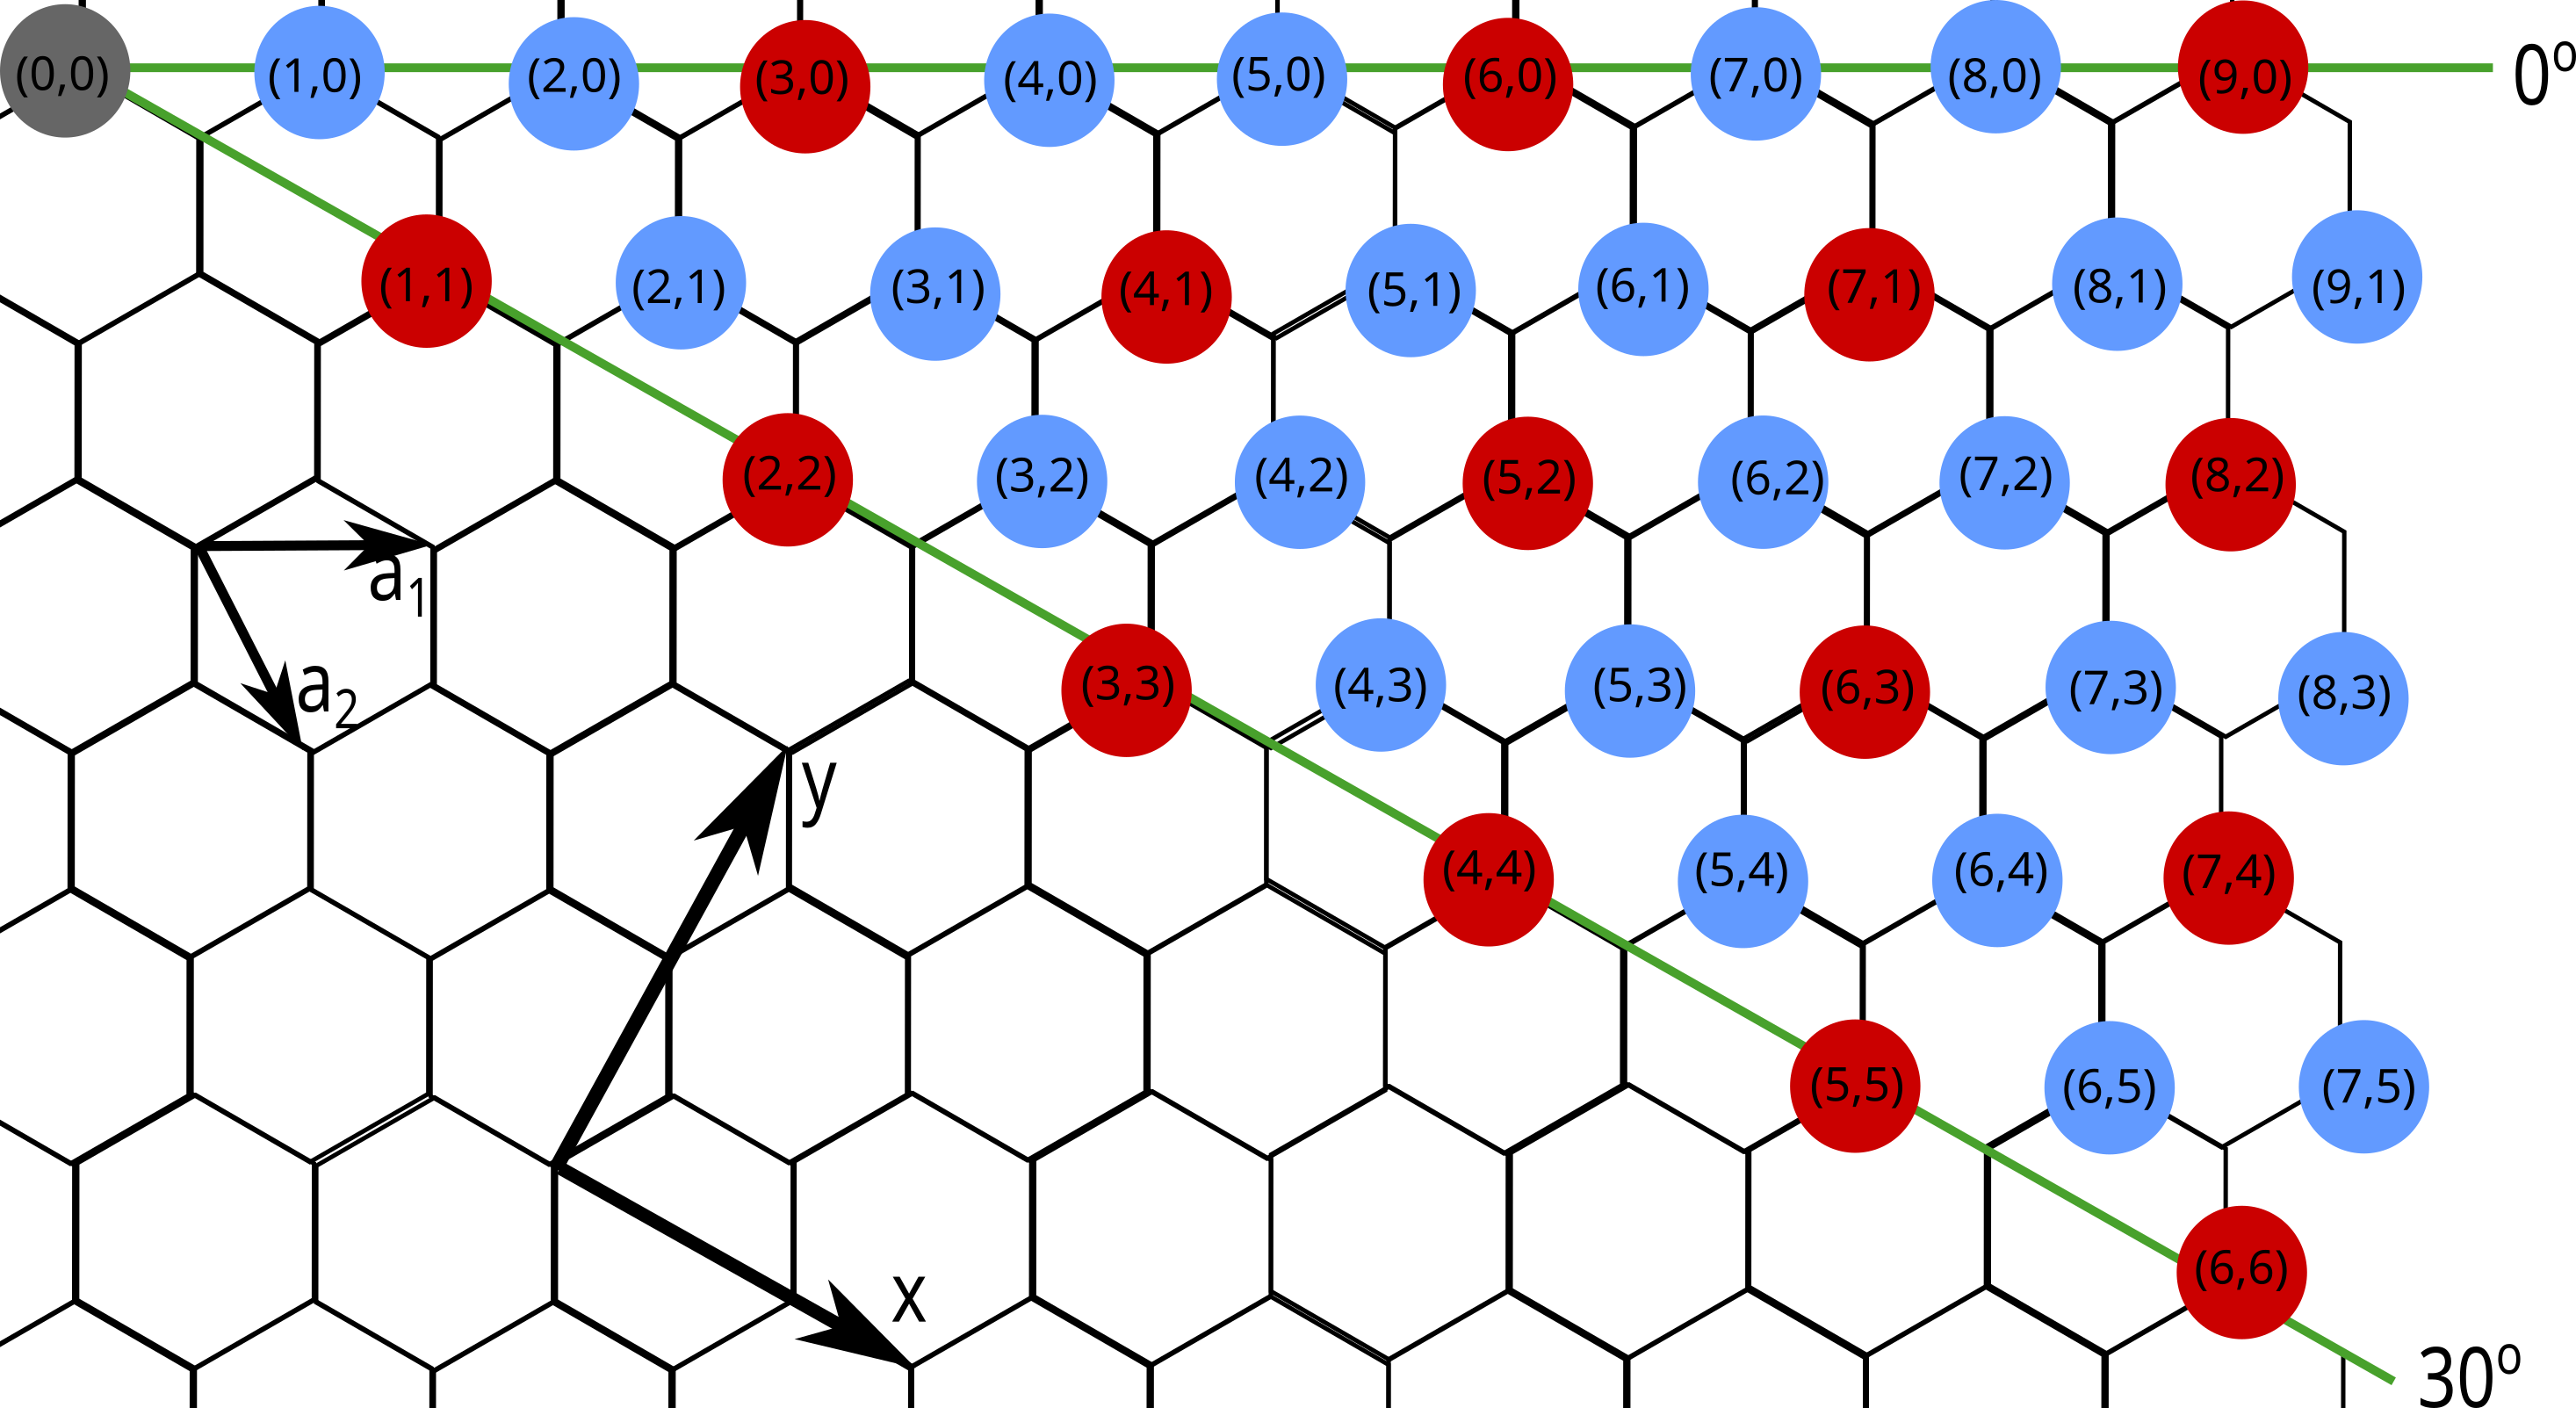
\includegraphics[width=0.8\textwidth]{./Figures/CNTs/chiral.png}
	\caption{Chiralities of CNTs with red dots indicating metallic and blue dots semiconductors. }
	\label{fig:chiralities}
\end{figure}
\section{Characterizing Carbon Nanotubes}
The main descriptive property of CNTs is the chiral vector, the  inter-valued scaling of the unit vectors for the honeycomb structure of graphene, written in the form (n, m).
\begin{equation}
	C_h = na_1 + ma_2 = (n, m)
\end{equation}
The unit vectors describing the lattice are of equal length and in Cartesian coordinates are defined
\begin{equation}
	a_1 = (\frac{\sqrt3}{2}, \frac{1}{2})\sqrt{3}a_{C-C}\\
	a_2 = (\frac{\sqrt3}{2}, -\frac{1}{2})\sqrt{3}a_{C-C}
	\label{unit_vecs}
\end{equation}
 where $a_{C-C}$ is the length of the carbon bond. For graphene,  $a_{C-C}$=1.421 (\AA) but for CNTs is approximately 1.44(\AA) with variation coming from the tube curvature\cite{saito}. From the chiral vector, much about the electronic and optical properties of individual CNTs can be inferred. The angle between the unit vectors, known as the chiral angle $\theta$, gives the direction of the chiral vector and the diameter,$d_t$, of the CNT are related to the chiral numbers:
\begin{equation}
	\theta = tan^{-1}\Bigg[\frac{m\sqrt{3}}{m + 2n}\Bigg]
\end{equation}
\begin{equation}
	d_t = \frac{a_{CC}\sqrt{3}}{\pi} \sqrt{n^2 + nm + m^2}
\end{equation}
The chiral angle is typically defined between 0${}^o$(a "zigzag" configuration) and 30${}^o$(an "armchair" configuration), labeled in Fig.\ref{fig:chiralities} due to the six-fold rotational symmetry lattice, as CNTs of mirrored chiral angles will have the sample opto-electrical properties. \\
As can be seen from the above definition, the tube diameter of CNTs is quantized. This quantization stems from the additional electron confinement around their circumference
\begin{equation}
	C_h\cdot\kappa = 2\pi q
\end{equation}
 as the cutting joining of the edges of graphene form the tubes only occurs at lines intersecting the lattice vertices. $\kappa$, the cutting line along the graphene energy bands, at integer value $q$ positions forms a the corresponding pattern of  metallic or a semiconductors \cite{dresselhaus} with all CNTs with a difference in chiral numbers $|m-n|$ that are multiples of 3 emerging as metallic. Work by H. Kataura et. al \cite{kataura} first plotted the energy differences between the van Hoven transitions, corresponding to the peaks in the conduction and valence bands enumerated starting from the Fermi energy, indicated in the 1D DOS plots in Fig.\ref{fig:kataura}(b)(c) later determined from \cite{saito}. The relationship of the first van Hoven transition to the diameter is found to be 
 \begin{equation}
 	E_{11} = \frac{2\gamma a_{C-C}}{d}
 \end{equation}
 is shown in Fig.\ref{fig:kataura}(a), with the average band gap energies split along semiconductor and metallic chiral values. The absorption peak wavelength of a nanotube sample is determined by the mean tube diameter, and the absorption spectral bandwidth will be determined by the tube diameter distribution of the CNT sample.
\begin{figure}[h]
	\centering
	\foreach \x \y in {kautura/0.7, dos\_66/0.47, dos\_76/0.47}
	{
		\begin{subfigure}[b]{0\y\textwidth}
			\includegraphics[width=\textwidth]{./Figures/CNTs/\x.png}
			\caption{}
		\end{subfigure}
		\hfil
	}
	\caption{(a)The Kataura plot, showing the relationship between CNT diameter and energy separation. Red dots indicate metallic and black semiconducting. The density of states for (b) Metallic and (c) Semiconducting CNTs and their energy band gaps. The green line indicates the Fermi level. Plots generated using data from\cite{maruyama}.}
	\label{fig:kataura}
\end{figure}
\clearpage
\subsubsection{Polarization Dependence}
Single isolated CNTs exhibit polarization dependence with the electric field in optical selection rules, i.e. the possible transitions from one quantum state to another \cite{thomsen}. Polarization dependence is only strong in zigzag-type nanotubes, the parity of the  dipole operator ( -1 in the horizontal plane dipole operator along the z-axis and +1the x-y plane) thus indicates absorption of light with the optical polarization parallel to the axial direction of the tube. However, in a bundle or random-oriented CNT grouping there will be no polarization dependence and it is not something that is of concern in CNTs dispersed in a solution.

\section{Nonlinear Optical Properties of CNTs}
The general relationship between the polarization and electric field of a material is defined \cite{yamashita} as
\begin{equation}
	P(t) = \epsilon_0(\chi^{(1)}E(t) + \chi^{(2)}E^2(t) + \chi^{(3)}E^3(t)+...)
\end{equation}
where $\chi^{(1)}$ is the linear susceptibility and $\chi^{(2)}$ and $\chi^{(3)}$are the second and third order susceptibility. Due to symmetry of the CNT’s structure, the second-order susceptibility is zero but a large third-order nonlinearity in CNTs has been measured \cite{martinez} and is theorized to be a product of the one dimensional motion of the delocalized $\pi$-band electrons at a fixed lattice ion configuration \cite{margulis}.  The third-order nonlinearity is responsible for the saturable absorption $\alpha$ of a material as well as the nonlinear Kerr effect.
The refractive index for such a material will be composed of the real part of the third-order susceptibility with $I$ defining the optical intensity, $n_0$  as the linear refractive index, $n_2$ and  is the nonlinear refractive index.
\begin{equation}
	n = n_0 + n_2I = n_0 + \frac{3Re[\chi^{(3)}]}{4\epsilon_0cn_0^2}I
	\label{eq:refractive_index}
\end{equation}
Saturable absorption is a phenomenon where high intensity light will reduce the absorption of a material, but at weak intensity, the light will be absorbed and cause attenuation. This property of materials with strong third-order susceptibility like CNTs can be used to filter out weaker optical signals in noisy optical pulses, while simultaneously allowing strong pulses to pass through. The absorption coefficient is composed of the imaginary part of the third-order susceptibility and $\alpha_0$, $\alpha_{int}$, and $\omega$ are the linear absorption coefficient, the non saturable absorption coefficient, and optical angular frequency respectively:
\begin{equation}
	\begin{aligned}
	\alpha &= \frac{\alpha_0}{1+\frac{I}{I_S}} + \alpha_{int}\\
	&\sim\alpha_0 + \alpha_{int} + \frac{3\omega Im[\chi^{3}]}{2\epsilon_0c^2n_0^2}I
	\end{aligned}
	\label{eq:absorption_coefficient}
\end{equation}
the saturation intensity$I_s$ is the power per unit area it takes in a steady state to reduce the absorption to half of completely saturated value, referred to as the unbleached state. Saturable absorption is observed in all materials with optical absorption resulting from electron transition between two energy levels \cite{thomsen}, but it is rare to find materials that have a recovery time that has a fast recovery time compared to the pulse duration. In bundles of  CNTs  with a variety of diameter sizes, entanglement between semiconducting and metallic via electrons tunneling and coupling from semiconducting CNTs to metallic CNTs \cite{gambetta} can result in picosecond to femtosecond range recovery time. Bundled CNTs have found application in  in ultra-fast laser applications where this sort of recovery time is needed, having been successful implemented in mode-locking femtosecond fiber-lasers\cite{fl1, fl2, fl3, fl4}. 

\section{Fluorescence of CNTs}
Arriving at the interest in CNTs for this thesis, semiconducting CNTs can be optically excited and emit fluorescence\cite{hendler} when well-dispersed. Bundled CNTs or placed on a substrate have little to no fluorescence at all, as interactions between CNTs cause increased quenching effects, the highest fluorescence quantum yields are seen in CNTs suspended in aqueous solutions. Though certain solvents mix better with certain chiralities CNTs to increase fluorescence, isolation to single chiralities one of the largest factors in increasing fluorescence. Desired type of CNTs can be targeted and isolated in a single step using modified aqueous two-phase extraction(ATPS)\cite{turek}.In this process, hydration modulating agents are mixed in to solutions to tune the arrangement of surfactants on their surface. Depending on the mixture, selected CNTs turn highly hydrophobic or hydrophilic, separating them from the rest of the mixture.\\
Fluorescence in carbon nanotubes is the product of absorption at the excitation frequency, corresponding to the second Van Hove optical transition (E22) , labeled in Fig.\ref{fig:kataura}(c), from the valence to conduction bands, followed by relaxation to the first Van Hove optical transition (E11) from the conduction to valence band. The corresponding excitation and emission  wavelengths can be as a function of diameter in nanometers and chiral angle are degrees derived in \cite{bachilo}. The parameters fitted differ along CNT groups, having to do with chiral number differences:  (n-m) mod 3 = 1 is group 1, (n-m) mod 3 = 2 is group 2,  (n-m) mod 3 = 0 are metallic CNTs and do not fluoresce and so are excluded. \\
For group 1:
\begin{equation}
	(Emission)\lambda_{11} = \Bigg[\frac{10^7(cm^{-1})}{157.5+1066.9d_t} - A_{1m1}(cm^{-1})\frac{cos(3\theta)^{1.374}}{d_t^{2.272}} \Bigg]^{-1}
\end{equation}
\begin{equation}
	(Excitation)\lambda_{22} = \Bigg[\frac{10^7(cm^{-1})}{145.6+575.7d_t} + A_{2m1}(cm^{-1})\frac{cos(3\theta)^{0.828}}{d_t^{1.809}} \Bigg]^{-1}
\end{equation}
For group 2:
\begin{equation}
	(Emission)\lambda_{11} = \Bigg[\frac{10^7(cm^{-1})}{157.5+1066.9d_t} + A_{1m2}(cm^{-1})\frac{cos(3\theta)^{0.886}}{d_t^{2.129}} \Bigg]^{-1}
\end{equation}
\begin{equation}
	(Excitation)\lambda_{22} = \Bigg[\frac{10^7(cm^{-1})}{145.6+575.7d_t} - A_{2m2}(cm^{-1})\frac{cos(3\theta)^{1.110}}{d_t^{2.497}} \Bigg]^{-1}
\end{equation}
Additional parameters $A_{1m1}, A_{1m2}, A_{2m1}, A_{2m2}$, account for variations of spectrum in same diameter CNTs. Not all variation differences are yet explained but comparison of aqueous solutions\cite{turek}\cite{weisman} found spectral shifts of ~2\%. \\
Plots of the excitation-emission spectrum are using variational parameters from fitting to data of samples of individual SWNT in aqueous sodium dodecyl sulfate (SDS)\cite{weisman} are shown in Fig.\ref{fig:cnt fluorescence}. Group 1 CNTs have lower Stokes shifts, and small chiral angles ($< 2^o$) while group 2 have higher Stokes shift and span full $0^o$to $30^o$ chiral angle range with similar angles along chiral number difference $(n - m)$. Regardless of group, the in excitation and emission wavelengths increase with diameter.
\begin{figure}[h]
	\centering
	\foreach \x in {degrees, diameter}
		{
			\begin{subfigure}[b]{0.49\textwidth}
				\includegraphics[width=9cm, height=8cm]{./Figures/CNTs/\x.png}
				\caption{}
			\end{subfigure}
			\hfil
		}
	\caption {Group characteristics of CNTs colored by using variational parameters from\cite{weisman}, valid for diameters $>0.5nm$. Color spectrum of plot denoting (a)chiral angle and (b)diameter. Increase in Stokes shifts with diameter along chiral difference $(n - m)$ lines, noted in red and connected by black lines.}
	\label{fig:cnt fluorescence}
\end{figure}
\clearpage
%======================================================================
\chapter{Optical Excitation of Semiconductor Nanoparticles in Hollow-Core Fiber}

% TODO: why is this in its own chapter. For ICG, background and results are in the same chapter. It would make 
% sense if it's the same for CNT. Also, a chapter with one single section is weird.

In this chapter we describe our experimental setup and procedures, as well as the results we obtained when studing the absorbance of semiconducting CNTs in liquid-filled HCPCF.

%======================================================================
\section{Bandgap Overlap}
Table shows all hollow-core fiber types available from ThorLabs and the central operating wavelengths for air-filled and D${}_2$O-filled fibers.
The “air” range can be used for fibers that are selectively core-filled with D${}_2$O.
The ranges for HC1550 and HC800B are approximated from spectrum measurements and HC2000 and HC1060 are taken from ThorLabs datasheets.
The D${}_2$O central wavelengths are calculated using the band-gap shift equation.

\begin{tabularx}{0.8\textwidth} { 
		| >{\centering\arraybackslash}X 
		| >{\centering\arraybackslash}X 
		| >{\centering\arraybackslash}X 
		| >{\centering\arraybackslash}X | }
	\hline
	HCPCF & $\lambda_{AIR}$ (nm) & $\lambda_{D_2O}$(nm) & Range (nm)\\
	\hline
	HC2000 & 2000 & 1144 & 250\\
	\hline
	HC1550 & 1550 & 887 & 500\\
	\hline
	HC1060 & 1060 & 606& 100\\
	\hline
	HC800B & 800 & 457 & 200\\
	\hline	
\end{tabularx}
\captionof{table}{ Thorlabs fiber bandgap shift. \label{bgoverlap}}

\begin{figure}[h]
	\centering
	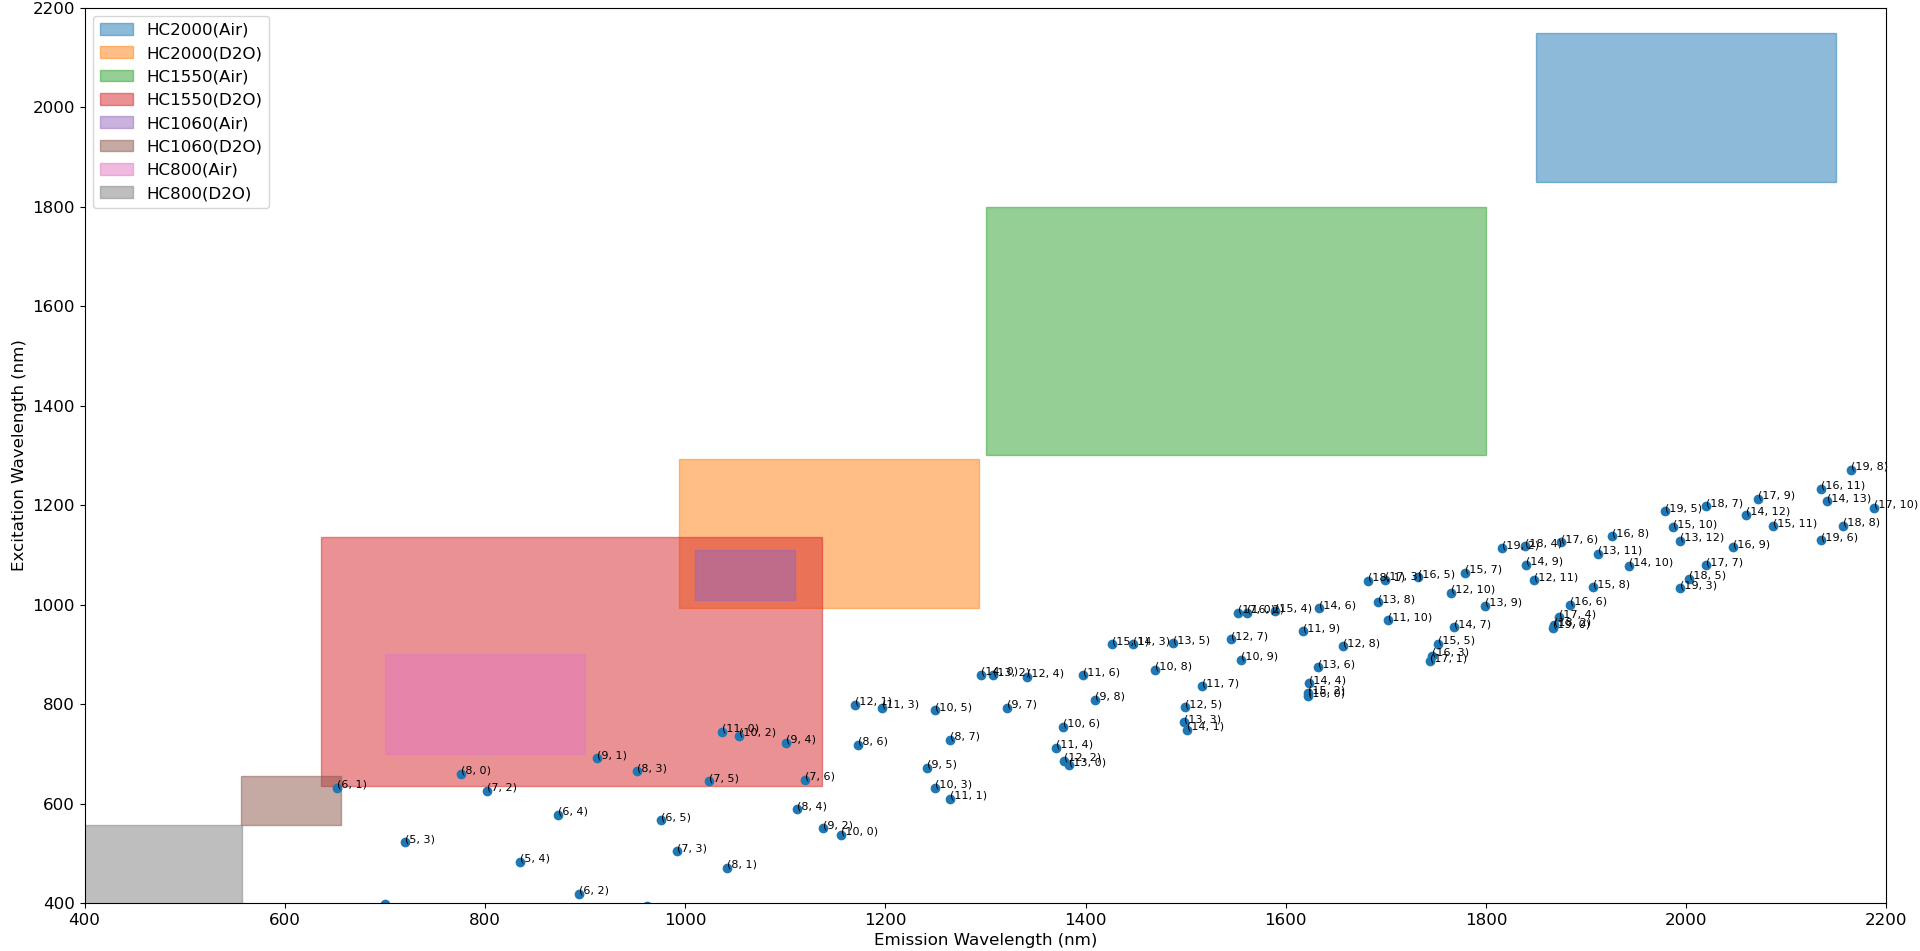
\includegraphics[width=\textwidth]{./Figures/CNTs/fibers_cnt.png}
	\caption{ Hollow-core fiber bandgap overlayed on CNT emission vs. excitation wavelengths }
	\label{fig:cntoverlap}
\end{figure}

\begin{figure}[h]
	
	\begin{minipage}{0.55\linewidth}
		\begin{tabularx}{\linewidth} { 
				| >{\centering\arraybackslash}X 
				| >{\centering\arraybackslash}X 
				| >{\centering\arraybackslash}X 
				| >{\centering\arraybackslash}X 
				| >{\centering\arraybackslash}X
				| >{\centering\arraybackslash}X
				| >{\centering\arraybackslash}X | }
			\hline
			$(n,m)$ & $dt$ (nm)	& $\Theta$ (deg) & 	$\lambda_{11}$ (nm)	 & $\lambda_{22}$ (nm)\\
			\hline
			(6, 1) & 0.52 & 0.13 & 652.62 & 631.79\\
			\hline
			(7, 2) & 0.65 & 0.21 & 802.05 & 625.92\\
			\hline
			(7, 5) & 0.83 & 0.43 & 1023.74 & 645.33\\
			\hline
			(7, 6)  & 0.89 & 27.46 & 1119.76 & 647.64\\
			\hline
			(8, 0) & 0.64 & 0 & 776.01 & 660.25\\
			\hline
			(8, 3) & 0.78 & 0.27 & 951.61 & 665.39\\
			\hline
			(9, 1) & 0.76 & 0.09 & 912.1 & 691.29\\
			\hline
			(9, 4)  & 0.92 & 0.31 & 1100.63 & 722.39\\
			\hline
			(10, 2) & 0.88 & 0.16 & 1053.43 & 736.68\\
			\hline
			(11, 0)  & 0.87 & 0 & 1036.93 & 744.57\\
			\hline
		\end{tabularx}
		\captionof{table}{ CNTs with emission and excitation transmittable through HC1550 filled with D${}_2$O. \label{cnt1550}}
	\end{minipage}
	\begin{minipage}{0.44\linewidth}
		\centering
		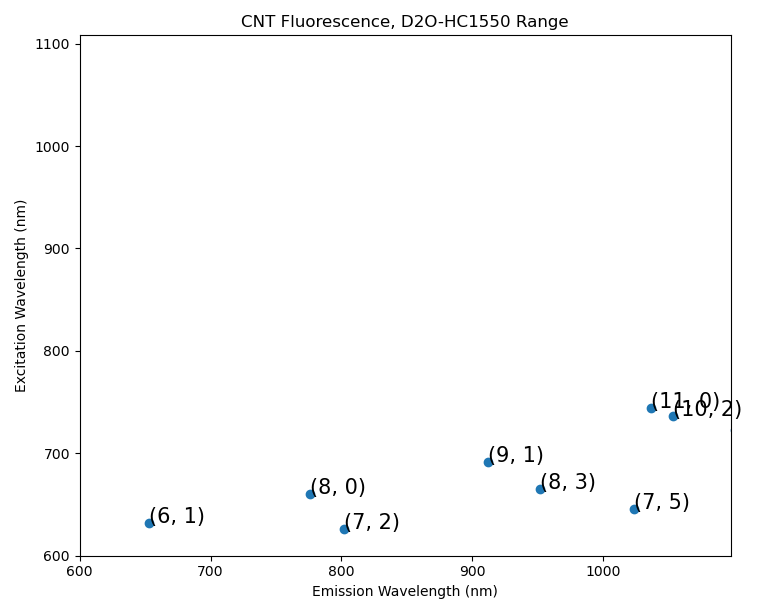
\includegraphics[width=9cm,height=7cm]{./Figures/CNTs/HC1550_range.png}
		\caption{ 1550HC CNTs }
		\label{fig:cnt1550}
	\end{minipage}
\end{figure}
\clearpage

\subsection{Experiment Set-Up}
A tunable, few nanometer linewidth light source for excitation wavelengths between $600-700$nm was made by  passing a super continuum source through a diffraction grating and filtering through an optical slit. The full set-up used to measure absorption and fluorescence of the sample is shown in Fig.\ref{fig:cnt_setup}. 
\begin{figure}[htb!]
	\foreach \x \y in {CNT\_Abs\_SetUp/0.6, pickoff/0.4,CNT\_Fluor\_SetUp/0.6}
	{ 
		\begin{subfigure}[b]{\y\textwidth}
			\includegraphics[width=\textwidth]{./Figures/CNT_Measured/\x.png}
			\caption{}
		\end{subfigure}
		\hfil
	}
	\caption{The experiential used set-up for measuring (a)Absorption and (c) Fluorescence of CNT samples in a cuvette. (b)The spectrum and intensity of the excitation beam at $\lambda=645$nm  picked-offed the super continuum source. The power measures $~48\mu$W and fwhm$=6$nm.}
	\label{fig:cnt_setup}
\end{figure}

\subsubsection{Sample History}
CNT samples were prepared by HeeBong Yang from the QuIN Lab at the University of Waterloo. SG65i powder was purchased from Sigma Aldrich and Dispersed in a surfactant at an initial powder concentration of 1 mg/mL. The sample then underwent a procedure of purification steps, sorting with polymers \& surfactants, and polymer exchange. The final condition of the sample was 65\% (7,5), (7,6) dominant SWCNTs in DI water with 0.04\% DOC, but at an unknown concentration.
\subsubsection{Sample Characteristics}
CNT solutions follow Beer-Lambert's Law \cite{schoppler, jeong}, $A = log(\frac{I_{in}}{I_{out}}) = \varepsilon CL$ so the concentration can be deduced from the measured absorbance. Fig.\ref{fig:cnt_abs}(a) and the average previously reported extinction coefficient\cite{blanch, anson, jeong} $\varepsilon= 30.98$ mL mg${}^{-1}$cm${}^{-1}$  estimate a sample concentration around $0.0042\pm 0.0007$ mg/mL.

\begin{figure}[h]
	\centering
	\foreach \x in {OD, time}
	{ 
		\begin{subfigure}[b]{0.45\textwidth}
			\includegraphics[width=\textwidth]{./Figures/CNT_Measured/\x.png}
			\caption{}
		\end{subfigure}
		\hfil
	}
	\caption{(a) Absorbance spectrum of CNT sorted CNT sample (b)Absorbance of CNT sorted sample over 60 minutes, the absorbance of the sample stabilizes after 30 minutes.}
	\label{fig:cnt_abs}
\end{figure}
Unfortunately no PL was detected from the sample. Despite the high absorption loss from DI water in the excitation wavelength range, fluorescence has been detected for these chiralities of CNTs suspended in DI water before\cite{wei}, though there is 23.25\% pm 10\% decrease in PL intensity when using H${}_2$O instead of D${}_2$O for (7, 5) and 42.5\% pm 5\% for (7,6) \% and quantum yields are expected to be around 1.04\% and 1.40\% respectively. The next steps to preclude the source of  quenching in the CNT sample is to measure the absorption with various thicknesses of cuvette or to incrementally dilute the sample.
\clearpage

%======================================================================
\chapter{Conclusion}
%======================================================================
In this thesis use of  HCPCFs as a liquid-waveguide was studied. The preservation of light bandgap guidance through liquid demonstrated by experimentally confirming the scaling laws for liquid-filled fibers of H${}_2$O and D${}_2$O.
The main results of the thesis were obtained in the measurements of the interaction of suspended ICG particles within the mode of the fiber. The dye molecules were excited in the fiber and fully-filled HCPCF guiding light via optical bandgap exhibited a higher efficiency than that seen in the liquid-core fiber. Despite difficulty with the coupling, there is high enough efficiency the potential of creating fluorescent light sources .\\

According to the CNT spectrum calculations, there is some overlap for common commercially available HCPCF, 1550nm HCPCF is the most practical fiber, because it has the only bandgap that overlaps with the absorption and emission spectrum of several chiralities.\\

While the results of suspended ICG particles are promising and show a proof-of-concept, the progression to suspended CNTs in HCPCF is incomplete. The initial tests with a sorted CNTs sample were inconclusive and further inverstigations are needed to produce a high-fluorescence sample. Future experimental efforts will hopefully lead to uses of CNTs in fiber-integrated devices. Besides the CNT samples, one of the main challenges that remains is obtaining a consistent and high coupling to the 1550nm HCPCF. Butt-coupled mechanical splicing chips fabricated for 800nm HCPCF consistently achieve coupling around 75-80\% and robustly hold the fibers together\cite{maruf}, but the same recipe does not produce high-fidelity butt-coupled mechanical splicing chips for 1550nm HCPCF. This is another avenue that needs to be explored but we are confident that it can be solved with modest efforts.\\

\subsection{Future Work}
what is ECDL
fiber-integration 
diagram
advantages.


%----------------------------------------------------------------------
% END MATERIAL
% Bibliography, Appendices, Index, etc.
%----------------------------------------------------------------------

% Bibliography

% The following statement selects the style to use for references.  
% It controls the sort order of the entries in the bibliography and also the formatting for the in-text labels.
\bibliographystyle{plain}
% This specifies the location of the file containing the bibliographic information.  
% It assumes you're using BibTeX to manage your references (if not, why not?).
\cleardoublepage % This is needed if the "book" document class is used, to place the anchor in the correct page, because the bibliography will start on its own page.
% Use \clearpage instead if the document class uses the "oneside" argument
\phantomsection  % With hyperref package, enables hyperlinking from the table of contents to bibliography             
% The following statement causes the title "References" to be used for the bibliography section:
\renewcommand*{\bibname}{References}

% Add the References to the Table of Contents
\addcontentsline{toc}{chapter}{\textbf{References}}

%\bibliography{}
\begin{thebibliography}{99}
%HCPCF Background
\bibitem{yariv} Yariv, Amnon and Pochi Albert Yeh, Optical Waves in Crystals: Propagation and Control of Laser Radiation,”1st ed. Wiley-Interscience, 2002.
\bibitem{joannopoulos} J. D. Joannopoulos, Photonic crystals: molding the flow of light, 2nd ed. Princeton: Princeton University Press, 2008.
\bibitem{chourasia}R. K. Chourasia and V. Singh, “Estimation of photonic band gap in the hollow core cylindrical multilayer structure,” Superlattices and Microstructures, vol. 116, pp. 191–199, Apr. 2018, doi: 10.1016/j.spmi.2018.02.023.
\bibitem{villeneuve} P. R. Villeneuve and M. Piche´, “Photonic band gaps in two-dimensional square and hexagonal lattices,” Phys. Rev. B, vol. 46, no. 8, pp. 4969–4972, Aug. 1992, doi: 10.1103/PhysRevB.46.4969.
\bibitem{cregan}R. F. Cregan et al., “Single-Mode Photonic Band Gap Guidance of Light in Air,” Science, vol. 285, no. 5433, pp. 1537–1539, Sep. 1999, doi: 10.1126/science.285.5433.1537.
\bibitem{sukhoivanov} I. A. Sukhoivanov and I. V. Guryev, Photonic Crystals: Physics and Practical Modeling, vol. 152. Berlin, Heidelberg: Springer Berlin Heidelberg, 2009. doi: 10.1007/978-3-642-02646-1.
\bibitem{birks} T. A. Birks, D. M. Bird, T. D. Hedley, J. M. Pottage, and P. St. J. Russell, “Scaling laws and vector effects in bandgap-guiding fibres,” Opt. Express, vol. 12, no. 1, p. 69, 2004, doi: 10.1364/OPEX.12.000069.
\bibitem{antonopoulos} G. Antonopoulos, F. Benabid, T. A. Birks, D. M. Bird, J. C. Knight, and P. St. J. Russell, “Experimental demonstration of the frequency shift of bandgaps in photonic crystal fibers due to refractive index scaling,” Opt. Express, vol. 14, no. 7, p. 3000, 2006, doi: 10.1364/OE.14.003000.
%fiberfilling
\bibitem{maruf} R. A. Maruf and M. Bajcsy, “On-chip splicer for coupling light between
photonic crystal and solid-core fibers,” Appl. Opt., vol. 56, no. 16, p.
4680, Jun. 2017.
\bibitem{xiao} L. Xiao, W. Jin, M. S. Demokan, H. L. Ho, Y. L. Hoo, and C. Zhao,
“Fabrication of selective injection microstructured optical fibers with a
conventional fusion splicer,” Opt. Express, vol. 13, no. 22, p. 9014, 2005.
\bibitem{kedenburg} S. Kedenburg, M. Vieweg, T. Gissibl, and H. Giessen, “Linear refractive
index and absorption measurements of nonlinear optical liquids in the
visible and near-infrared spectral region,” Opt. Mater. Express, vol. 2,
no. 11, p. 1588, Nov. 201

%Modecoupling
\bibitem{bajcsy} M. Bajcsy et al., “Laser-cooled atoms inside a hollow-core photonic-crystal fiber,” Phys. Rev. A, vol. 83, no. 6, p. 063830, Jun. 2011, doi: 10.1103/PhysRevA.83.063830. 
\bibitem{hilton} A. P. Hilton, C. Perrella, F. Benabid, B. M. Sparkes, A. N. Luiten, and P. S. Light, “High-efficiency cold-atom transport into a waveguide trap,” Phys. Rev. Applied, vol. 10, no. 4, p. 044034, Oct. 2018, doi: 10.1103/PhysRevApplied.10.044034. A
\bibitem{domokos} P. Domokos, P. Horak, and H. Ritsch, “Quantum description of light-pulse scattering on a single atom in waveguides,” Phys. Rev. A, vol. 65, no. 3, p. 033832, Mar. 2002, doi: 10.1103/PhysRevA.65.033832.
\bibitem{mazoni} M. T. Manzoni, “New Systems for Quantum Nonlinear Optics,”. 2017, Thesis, p. 39-40.

%ICG
\bibitem{Fang} X. Fang et al., “One-step condensation synthesis and characterizations of indocyanine green,” Results in Chemistry, vol. 3, p. 100092, Jan. 2021, doi: 10.1016/j.rechem.2020.100092.
\bibitem{holzer}W. Holzer et al., "Photostability and thermal stability of indocyanine green," Journal of Photochemistry and Photobiology B: Biology,  vol. 47, no. 2-3, pp. 155-164, Dec. 1998.
\bibitem{landsman}M. L. Landsman, G. Kwant, G. A. Mook, and W. G. Zijlstra, “Light-absorbing properties, stability, and spectral stabilization of indocyanine green,” Journal of Applied Physiology, vol. 40, no. 4, pp. 575–583, Apr. 1976.
\bibitem{mauerer}M. Mauerer, A. Penzkofer, and J. Zweck, “Dimerization, J-aggregation and J-disaggregation dynamics of indocyanine green in heavy water,” Journal of Photochemistry and Photobiology B: Biology, vol. 47, no. 1, pp. 68–73, Nov. 1998.
\bibitem{rotermund}F. Rotermund, R. Weigand, W. Holzer, M. Wittmann, and A. Penzkofer, “Fluorescence spectroscopic analysis of indocyanine green J aggregates in water,” Journal of Photochemistry and Photobiology A: Chemistry, vol. 110, no. 1, pp. 75–78, Oct. 1997.
\bibitem{philip}R. Philip, A. Penzkofer, W. Bäumler, R. M. Szeimies, and C. Abels, “Absorption and fluorescence spectroscopic investigation of indocyanine green,” Journal of Photochemistry and Photobiology A: Chemistry, vol. 96, no. 1–3, pp. 137–148, May 1996.
\bibitem{saxena}V. Saxena, M. Sadoqi, and J. Shao, “Degradation Kinetics of Indocyanine Green in Aqueous Solution,” Journal of Pharmaceutical Sciences, vol. 92, no. 10, pp. 2090–2097, Oct. 2003. 
\bibitem{farrakhova}D. Farrakhova et al., “Fluorescence imaging analysis of distribution of indocyanine green in molecular and nanoform in tumor model,” Photodiagnosis and Photodynamic Therapy, vol. 37, p. 102636, Mar. 2022, doi: 10.1016/j.pdpdt.2021.102636.
\bibitem{spartalis} E. Spartalis et al., “Intraoperative Indocyanine Green (ICG) Angiography for the Identification of the Parathyroid Glands: Current Evidence and Future Perspectives,” In Vivo, vol. 34, no. 1, pp. 23–32, 2020, doi: 10.21873/invivo.11741.
\bibitem{dedora}D. J. DeDora et al., “Sulfobutyl ether $\beta$-cyclodextrin and methyl $\beta$-cyclodextrin enhance and stabilize fluorescence of aqueous indocyanine green: Sulfobutyl Ether $\beta$-Cyclodextrin and METHYL $\beta$-Cyclodextrin,” J. Biomed. Mater. Res., vol. 104, no. 7, pp. 1457–1464, Oct. 2016, doi: 10.1002/jbm.b.33496.
\bibitem{weigand}R. Weigand, F. Rotermund, and A. Penzkofer, “Degree of aggregation of indocyanine green in aqueous solutions determined by Mie scattering,” Chemical Physics, vol. 220, no. 3, pp. 373–384, Aug. 1997, doi: 10.1016/S0301-0104(97)00150-X.
\bibitem{hiemenz} P. C. Hiemenz and R. D. Vold, “Particle size from the optical properties of flocculating carbon dispersions,” Journal of Colloid and Interface Science, vol. 21, no. 5, pp. 479–488, May 1966, doi: 10.1016/0095-8522(66)90046-8.

%Liquid waveguides
\bibitem{cox}A. J. Cox, A. J. DeWeerd, and J. Linden, “An experiment to measure Mie and Rayleigh total scattering cross sections,” American Journal of Physics, vol. 70, no. 6, pp. 620–625, Jun. 2002, doi: 10.1119/1.1466815.
\bibitem{vezenov}D. V. Vezenov, B. T. Mayers, D. B. Wolfe, and G. M. Whitesides, “Integrated fluorescent light source for optofluidic applications,” Appl. Phys. Lett., vol. 86, no. 4, p. 041104, Jan. 2005, doi: 10.1063/1.1850610.
\bibitem{bliss}C. L. Bliss, J. N. McMullin, and C. J. Backhouse, “Integrated wavelength-selective optical waveguides for microfluidic-based laser-induced fluorescence detection,” Lab Chip, vol. 8, no. 1, pp. 143–151, 2008, doi: 10.1039/B711601B.
\bibitem{conroy}R. S. Conroy, B. T. Mayers, D. V. Vezenov, D. B. Wolfe, M. G. Prentiss, and G. M. Whitesides, “Optical waveguiding in suspensions of dielectric particles,” p. 5.
%CNT Background
\bibitem{cusano}A. Cusano et al., “Optical probes based on optical fibers and single-walled carbon nanotubes for hydrogen detection at cryogenic temperatures,” Appl. Phys. Lett., vol. 89, no. 20, p. 201106, Nov. 2006, doi: 10.1063/1.2370292.
\bibitem{dresselhaus} S. Dresselhaus, “PHYSICS OF CARBON NANOTUBES,” Carbon, 33(7), 883-891, 1995.
\bibitem{popov} V. Popov, “Carbon nanotubes: properties and application,” Materials Science and Engineering: R: Reports, vol. 43, no. 3, pp. 61–102, Jan. 2004.
\bibitem{yamashita} S. Yamashita, “Nonlinear optics in carbon nanotube, graphene, and related 2D materials,” APL Photonics, vol. 4, no. 3, p. 034301, Mar. 2019.
\bibitem{saito}R. Saito, M. Fujita, G. Dresselhaus, and M. S. Dresselhaus, “Electronic structure of chiral graphene tubules,” Appl. Phys. Lett., vol. 60, no. 18, pp. 2204–2206, May 1992.
\bibitem{thomsen}C. Thomsen, S. Reich, and J. Maultzsch, Carbon Nanotubes: Basic Concepts and Physical Properties, 1st ed. Wiley, 2004. 
\bibitem{kataura} H. Kataura et al., “Optical properties of single-wall carbon nanotubes,” Synthetic Metals, vol. 103, no. 1–3, pp. 2555–2558, Jun. 1999.
\bibitem{saito} R. Saito, G. Dresselhaus, and M. S. Dresselhaus, “Trigonal warping effect of carbon nanotubes,” Phys. Rev. B, vol. 61, no. 4, pp. 2981–2990, Jan. 2000, doi: 10.1103/PhysRevB.61.2981.
\bibitem{maruyama} S. Maruyama, Fullerene and Carbon Nanotube Site [Online]. Available: http://www.photon.t.u-tokyo.ac.jp/~maruyama/nanotube.html
\bibitem{yamashita.tutorial} S. Yamashita, “A Tutorial on Nonlinear Photonic Applications of Carbon Nanotube and Graphene,” J. Lightwave Technol., vol. 30, no. 4, pp. 427–447, Feb. 2012.
\bibitem{gambetta}A. Gambetta et al., “Sub-100 fs two-color pump-probe spectroscopy of Single Wall Carbon Nanotubes with a 100 MHz Er-fiber laser system,” p. 8, 2008.
\bibitem{weisman} R. B. Weisman and S. M. Bachilo, “Dependence of Optical Transition Energies on Structure for Single-Walled Carbon Nanotubes in Aqueous Suspension: An Empirical Kataura Plot,” Nano Lett., vol. 3, no. 9, pp. 1235–1238, Sep. 2003.
\bibitem{bachilo} S. M. Bachilo, M. S. Strano, C. Kittrell, R. H. Hauge, R. E. Smalley, and R. B. Weisman, “Structure-Assigned Optical Spectra of Single-Walled Carbon Nanotubes,” Science, vol. 298, no. 5602, pp. 2361–2366, Dec. 2002. 
\bibitem{giordani}S. Giordani et al., “Debundling of Single-Walled Nanotubes by Dilution: Observation of Large Populations of Individual Nanotubes in Amide Solvent Dispersions,” J. Phys. Chem. B, vol. 110, no. 32, pp. 15708–15718, Aug. 2006.
\bibitem{martinez} A. Martinez and S. Yamashita, “Carbon Nanotube-Based Photonic Devices: Applications in Nonlinear Optics,” In: J. M. Marulanda, Ed., Carbon Nanotubes Applications on Electron Devices, InTech, 2011. 
\bibitem{margulis} Vl. A. Margulis and T. A. Sizikova, “Theoretical study of third-order nonlinear optical response of semiconductor carbon nanotubes,” Physica B: Condensed Matter, vol. 245, no. 2, pp. 173–189, Mar.1998.
\bibitem{turek} E. Turek, T. Shiraki, T. Shiraishi, T. Shiga, T. Fujigaya, and D. Janas, “Single-step isolation of carbon nanotubes with narrow-band light emission characteristics,” Sci Rep, vol. 9, no. 1, p. 535, Dec. 2019
\bibitem{fl1} M. Chernysheva et al., “Carbon nanotubes for ultrafast fibre lasers,” Nanophotonics, vol. 6, no. 1, pp. 1–30, Jan. 2017, doi: 10.1515/nanoph-2015-0156.
\bibitem{fl2} C. S. Goh et al., “Femtosecond mode-locking of a ytterbium-doped fiber laser using a carbon-nanotube-based mode-locker with ultra-wide absorption band,” in (CLEO). Conference on Lasers and Electro-Optics, 2005., Baltimore, MD, USA, 2005, pp. 1644-1646 Vol. 3. doi: 10.1109/CLEO.2005.202227.
\bibitem{fl3} K. Kieu and F. W. Wise, “All-fiber normal-dispersion femtosecond laser,” Opt. Express, vol. 16, no. 15, p. 11453, Jul. 2008, doi: 10.1364/OE.16.011453.
\bibitem{fl4} Y. Z. Pan, J. G. Miao, W. J. Liu, X. J. Huang, and Y. B. Wang, “Mode-locked ytterbium fiber lasers using a large modulation depth carbon nanotube saturable absorber without an additional spectral filter,” Laser Phys. Lett., vol. 11, no. 9, p. 095105, Sep. 2014, doi: 10.1088/1612-2011/11/9/095105.

%CNT Measured
\bibitem{HC2000}NKT Photonics, “2 $\mu$m Range Hollow Core Photonic Bandgap Fiber,”HC-2000-01.
\bibitem{HC1060}NKT Photonics, “Hollow Core Photonic Bandgap Fiber for 1060nm Range Applications,”HC-1060-02.
\bibitem{hendler}A. Hendler-Neumark and G. Bisker, “Fluorescent Single-Walled Carbon Nanotubes for Protein Detection,” Sensors, vol. 19, no. 24, p. 5403, Dec. 2019, doi: 10.3390/s19245403.
\bibitem{wei} X. Wei et al., “Photoluminescence Quantum Yield of Single-Wall Carbon Nanotubes Corrected for the Photon Reabsorption Effect,” p. 23.
\bibitem{schoppler} F. Schöppler et al., “Molar Extinction Coefficient of Single-Wall Carbon Nanotubes,” J. Phys. Chem. C, vol. 115, no. 30, pp. 14682–14686, Aug. 2011, doi: 10.1021/jp205289h.
\bibitem{blanch} A. J. Blanch, C. E. Lenehan, and J. S. Quinton, “Parametric analysis of sonication and centrifugation variables for dispersion of single walled carbon nanotubes in aqueous solutions of sodium dodecylbenzene sulfonate,” Carbon, vol. 49, no. 15, pp. 5213–5228, Dec. 2011, doi: 10.1016/j.carbon.2011.07.039.
\bibitem{anson} A. Ansón-Casaos, J. M. González-Domínguez, I. Lafragüeta, J. A. Carrodeguas, and M. T. Martínez, “Optical absorption response of chemically modified single-walled carbon nanotubes upon ultracentrifugation in various dispersants,” Carbon, vol. 66, pp. 105–118, Jan. 2014, doi: 10.1016/j.carbon.2013.08.048.
\bibitem{jeong}S. H. Jeong, K. K. Kim, S. J. Jeong, K. H. An, S. H. Lee, and Y. H. Lee, “Optical absorption spectroscopy for determining carbon nanotube concentration in solution,” Synthetic Metals, vol. 157, no. 13–15, pp. 570–574, Jul. 2007, doi: 10.1016/j.synthmet.2007.06.012.
\bibitem{tsyboulski} D. A. Tsyboulski, J.-D. R. Rocha, S. M. Bachilo, L. Cognet, and R. B. Weisman, “Structure-Dependent Fluorescence Efficiencies of Individual Single-Walled Carbon Nanotubes,” Nano Lett., vol. 7, no. 10, pp. 3080–3085, Oct. 2007, doi: 10.1021/nl071561s.
%Future Work
\bibitem{ding}K. Ding et al., “Research on Narrow Linewidth External Cavity Semiconductor Lasers,” Crystals, vol. 12, no. 7, p. 956, Jul. 2022, doi: 10.3390/cryst12070956.
\bibitem{duarte} F. J. Duarte, Ed., Organic Lasers and Organic Photonics, Bristol, IOP, 2018. doi: 10.1007/978-3-662-11579-4.
\bibitem{shafer}F. P. Schäfer, Ed., Dye Lasers, vol. 1. Berlin, Heidelberg: Springer Berlin Heidelberg, 1973. doi: 10.1007/978-3-662-11579-4.
\bibitem{pierce}B. Pierce and R. Birge, “Lasing properties of several near-IR dyes for a nitrogen laser-pumped dye laser with an optical amplifier,” IEEE J. Quantum Electron., vol. 18, no. 7, pp. 1164–1170, Jul. 1982, doi: 10.1109/JQE.1982.1071672.
\bibitem{norwood} Robert A. Norwood, "Organic Photonics: Ready for Prime Time," Optics \& Photonics News 24(11), 40-47, 2013.
\bibitem{stuke}M. Stuke, Dye Lasers: 25 Years. Berlin, Heidelberg: Springer-Verlag Springer, ch.11, 2005. 

\end{thebibliography}

% Tip: You can create multiple .bib files to organize your references. 
% Just list them all in the \bibliogaphy command, separated by commas (no spaces).

% The following statement causes the specified references to be added to the bibliography even if they were not cited in the text. 
% The asterisk is a wildcard that causes all entries in the bibliographic database to be included (optional).
\nocite{*}
%----------------------------------------------------------------------

% Appendices

% The \appendix statement indicates the beginning of the appendices.
\appendix
% Add an un-numbered title page before the appendices and a line in the Table of Contents
%\chapter*{APPENDICES}
%\addcontentsline{toc}{chapter}{APPENDICES}
% Appendices are just more chapters, with different labeling (letters instead of numbers).
%\label{AppendixA}
% Tip 4: Example (above) of how to get a shorter chapter title for the Table of Contents 
%======================================================================
\section{CNT Sample Preparation }
•Sample history
1) SG65i powder purchased from Sigma Aldrich
2) Dispersed in a surfactant
3) Purification steps
4) Sorting with polymers \& surfactants
5) Polymer exchange
6) UV-vis measurements
-. (7,5), (7,6) dominant: 65 \% in the sample
-. Semiconducting: > 99 \%

• Sample Condition
-. SWCNTs are in DI water with DOC 0.04\%
-. Greenish color
-. Amount: 1 mL

%----------------------------------------------------------------------
\end{document} % end of logical document
